\chapter{Calibración de los sensores}
%%%%%%%%%%%%%%%%%%%%%%%%%%%%%%%%%%%%%%%%%%%%%%%%%%%%%%%%%%%%%%%%%%%%%%%%%%%%%%%%%%%%%%%%%%%%%%%%%%%%%%

Con objeto de facilitar la configuración de los sensores analógicos, se han habilitado 4 botones al equipo.

\begin{figure}[htbp!] 
\centering{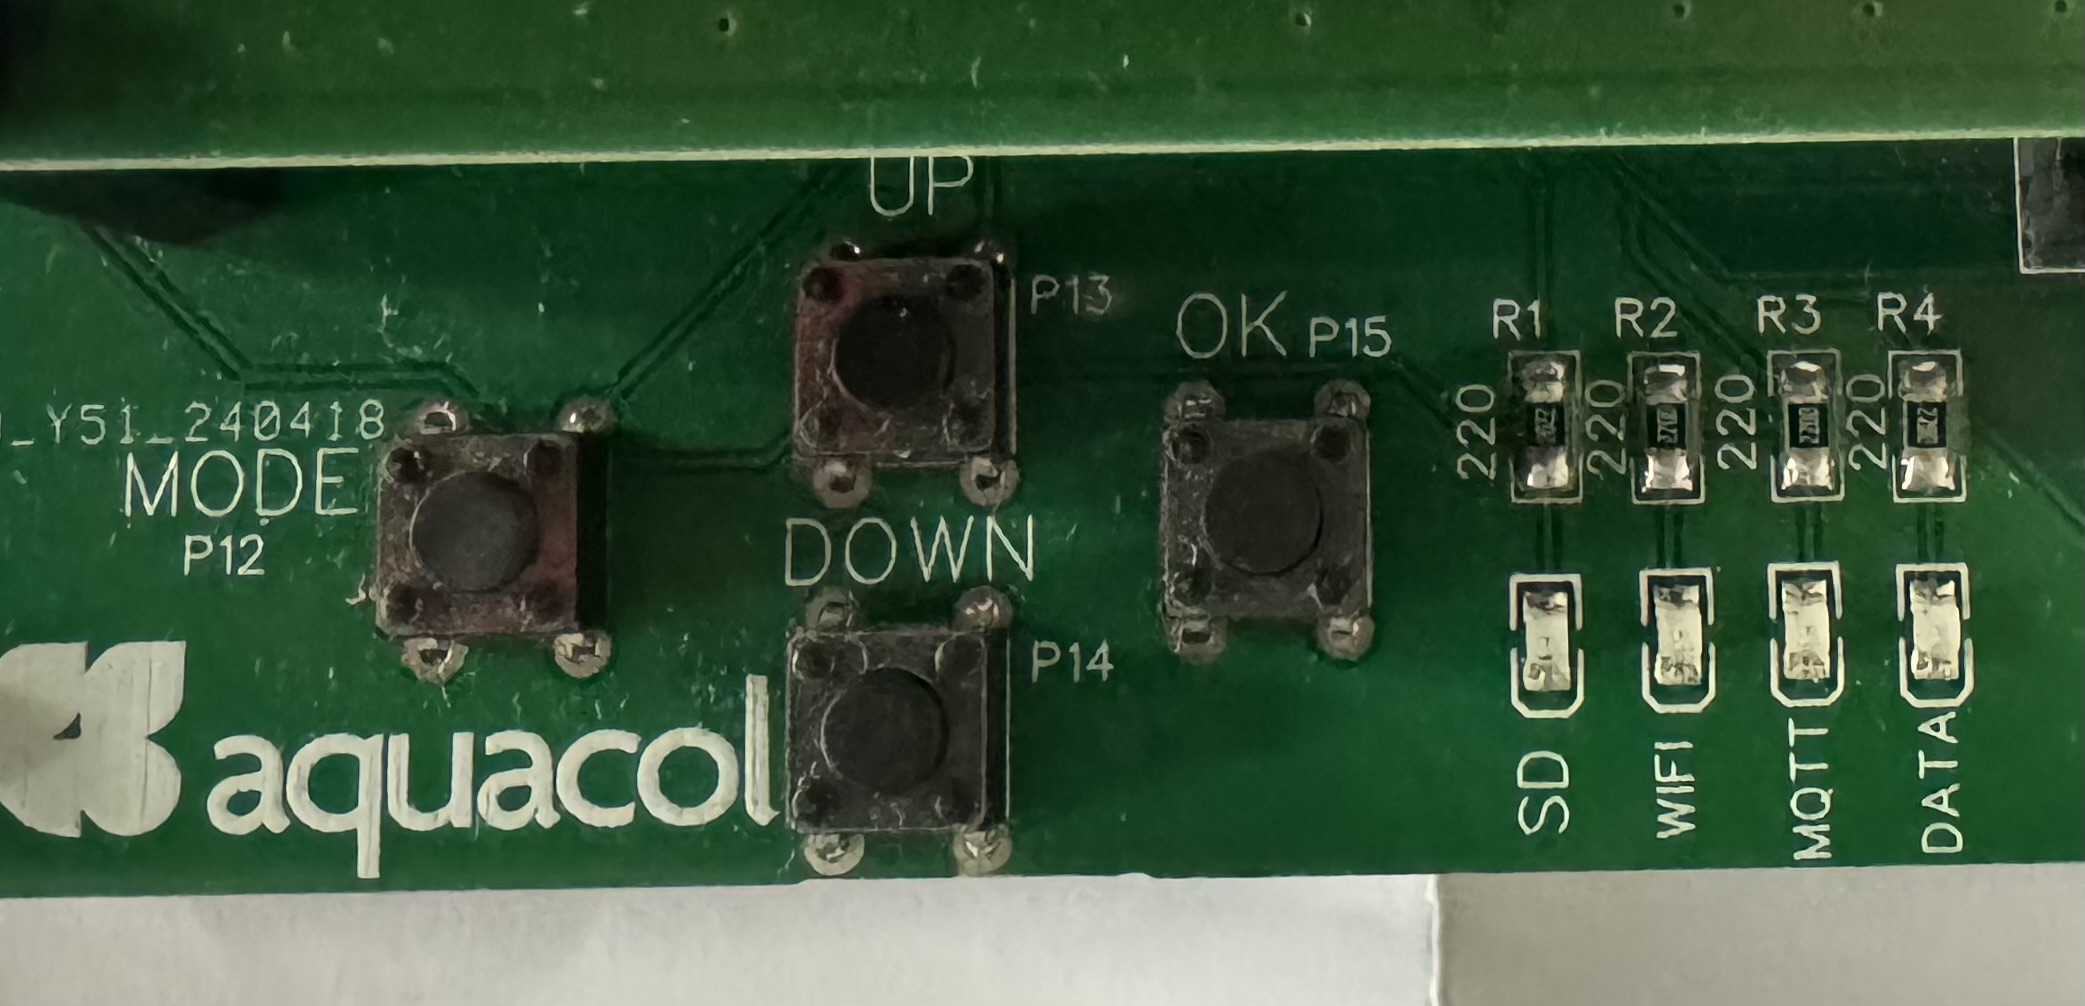
\psfig{file=Figuras/Botones.jpeg,width=10cm,angle=0}} 
\caption{Botones y leds de estado}\label{botones} 
\end{figure}

Puede ver que hay 4 botones
\begin{itemize}
\item \textbf{MODE}. Nos sirve para cambiar de pantalla.
\item \textbf{UP}. Nos sirve para subir determinado parámetro en la calibración. Va a depender de la pantalla en la que se esté.
\item \textbf{DOWN}. Nos sirve para bajar determinado parámetro en la calibración. Va a depender de la pantalla en la que se esté.
\item \textbf{OK}. Guardará la configuración de del parámetro en el archivo \emph{config.txt} y volverá a la pantalla por defecto.
\end{itemize}

Los botones puede parecer que a veces no funcionan, es normal. Es debido a un problema de rebotes (falsos contactos) se está trabajando en solucionarlo. No se pulsan solos , solo a veces no detecta que se pulsan.

\section{Secuencia de arranque}

Cuando arranca el equipo pasa por una serie de pantallas:
\begin{enumerate}
\item Primero configura la tarjeta microSD, es importante que esta parte funcione porque en la tarjeta está toda la información de la WIFI y de configuración de los sensores. Se encenderá el led con la etiqueta SD de la figura \ref{botones}.

En caso de que la tarjeta microSD no esté bien configurada (ver figura \ref{patalla:Nosd}), ya sea porque el formato no es el correcto (FAT 32), porque no está bien pinchada en el alojamiento o porque no exista en la tarjeta el archivo \emph{config.txt}. 

\begin{figure}[htbp!] 
\centering{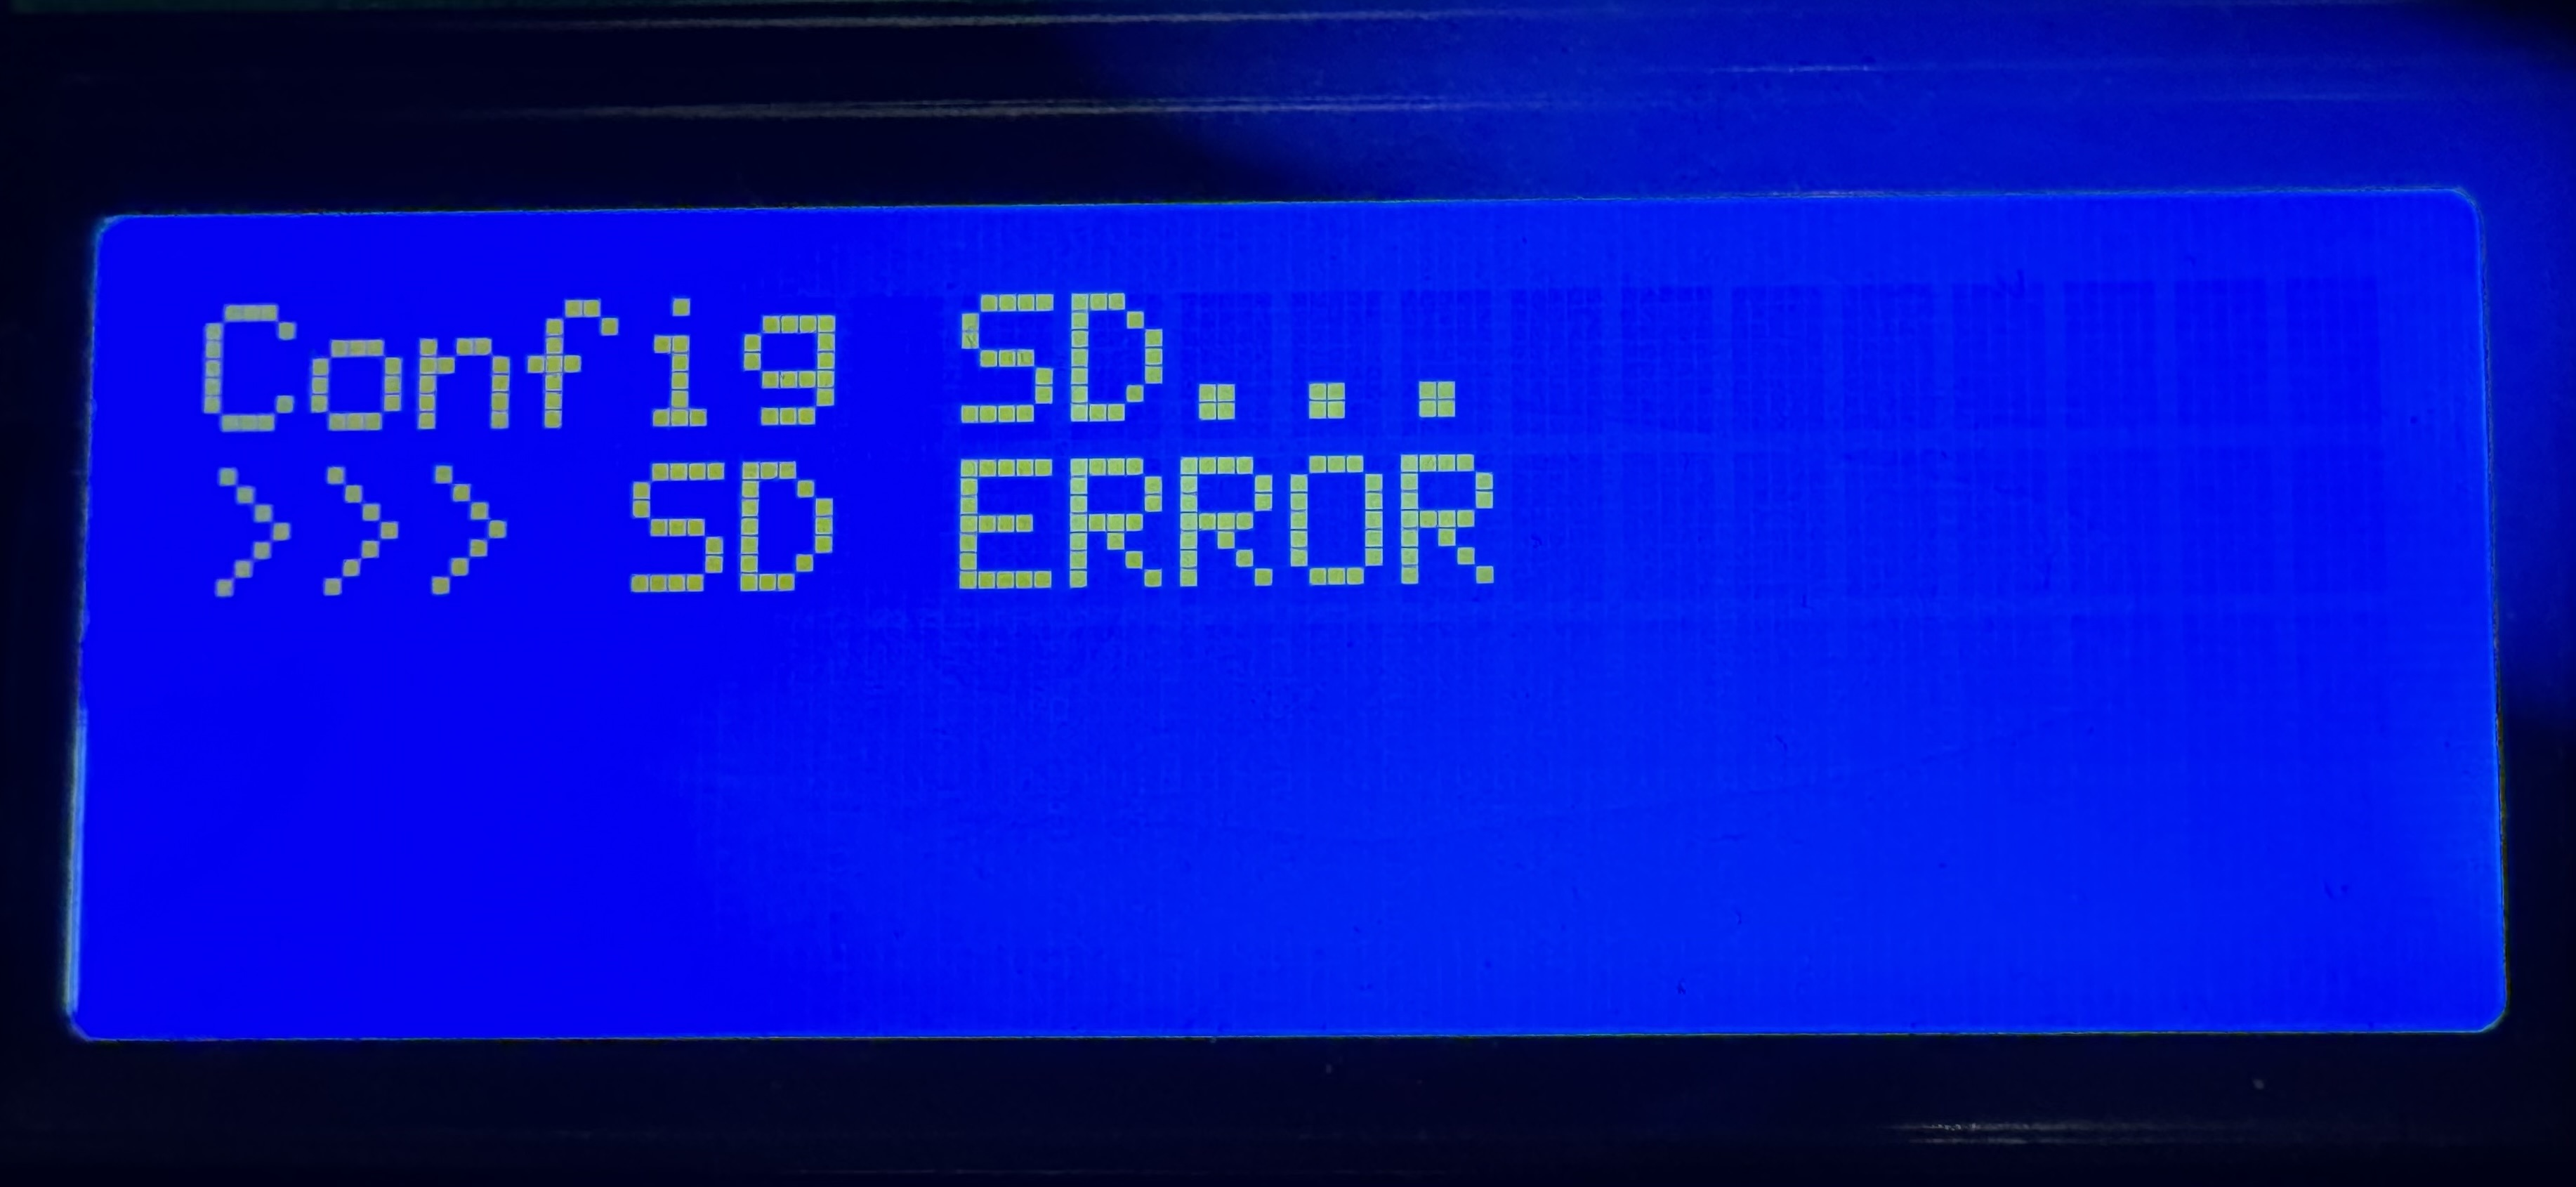
\psfig{file=Figuras/SD_ERROR.jpeg,width=8cm,angle=0}} 
\caption{SD ERROR}\label{patalla:Nosd} 
\end{figure}

Se cargará la configuración por defecto (figura \ref{patalla:condef} )  

\begin{figure}[htbp!] 
\centering{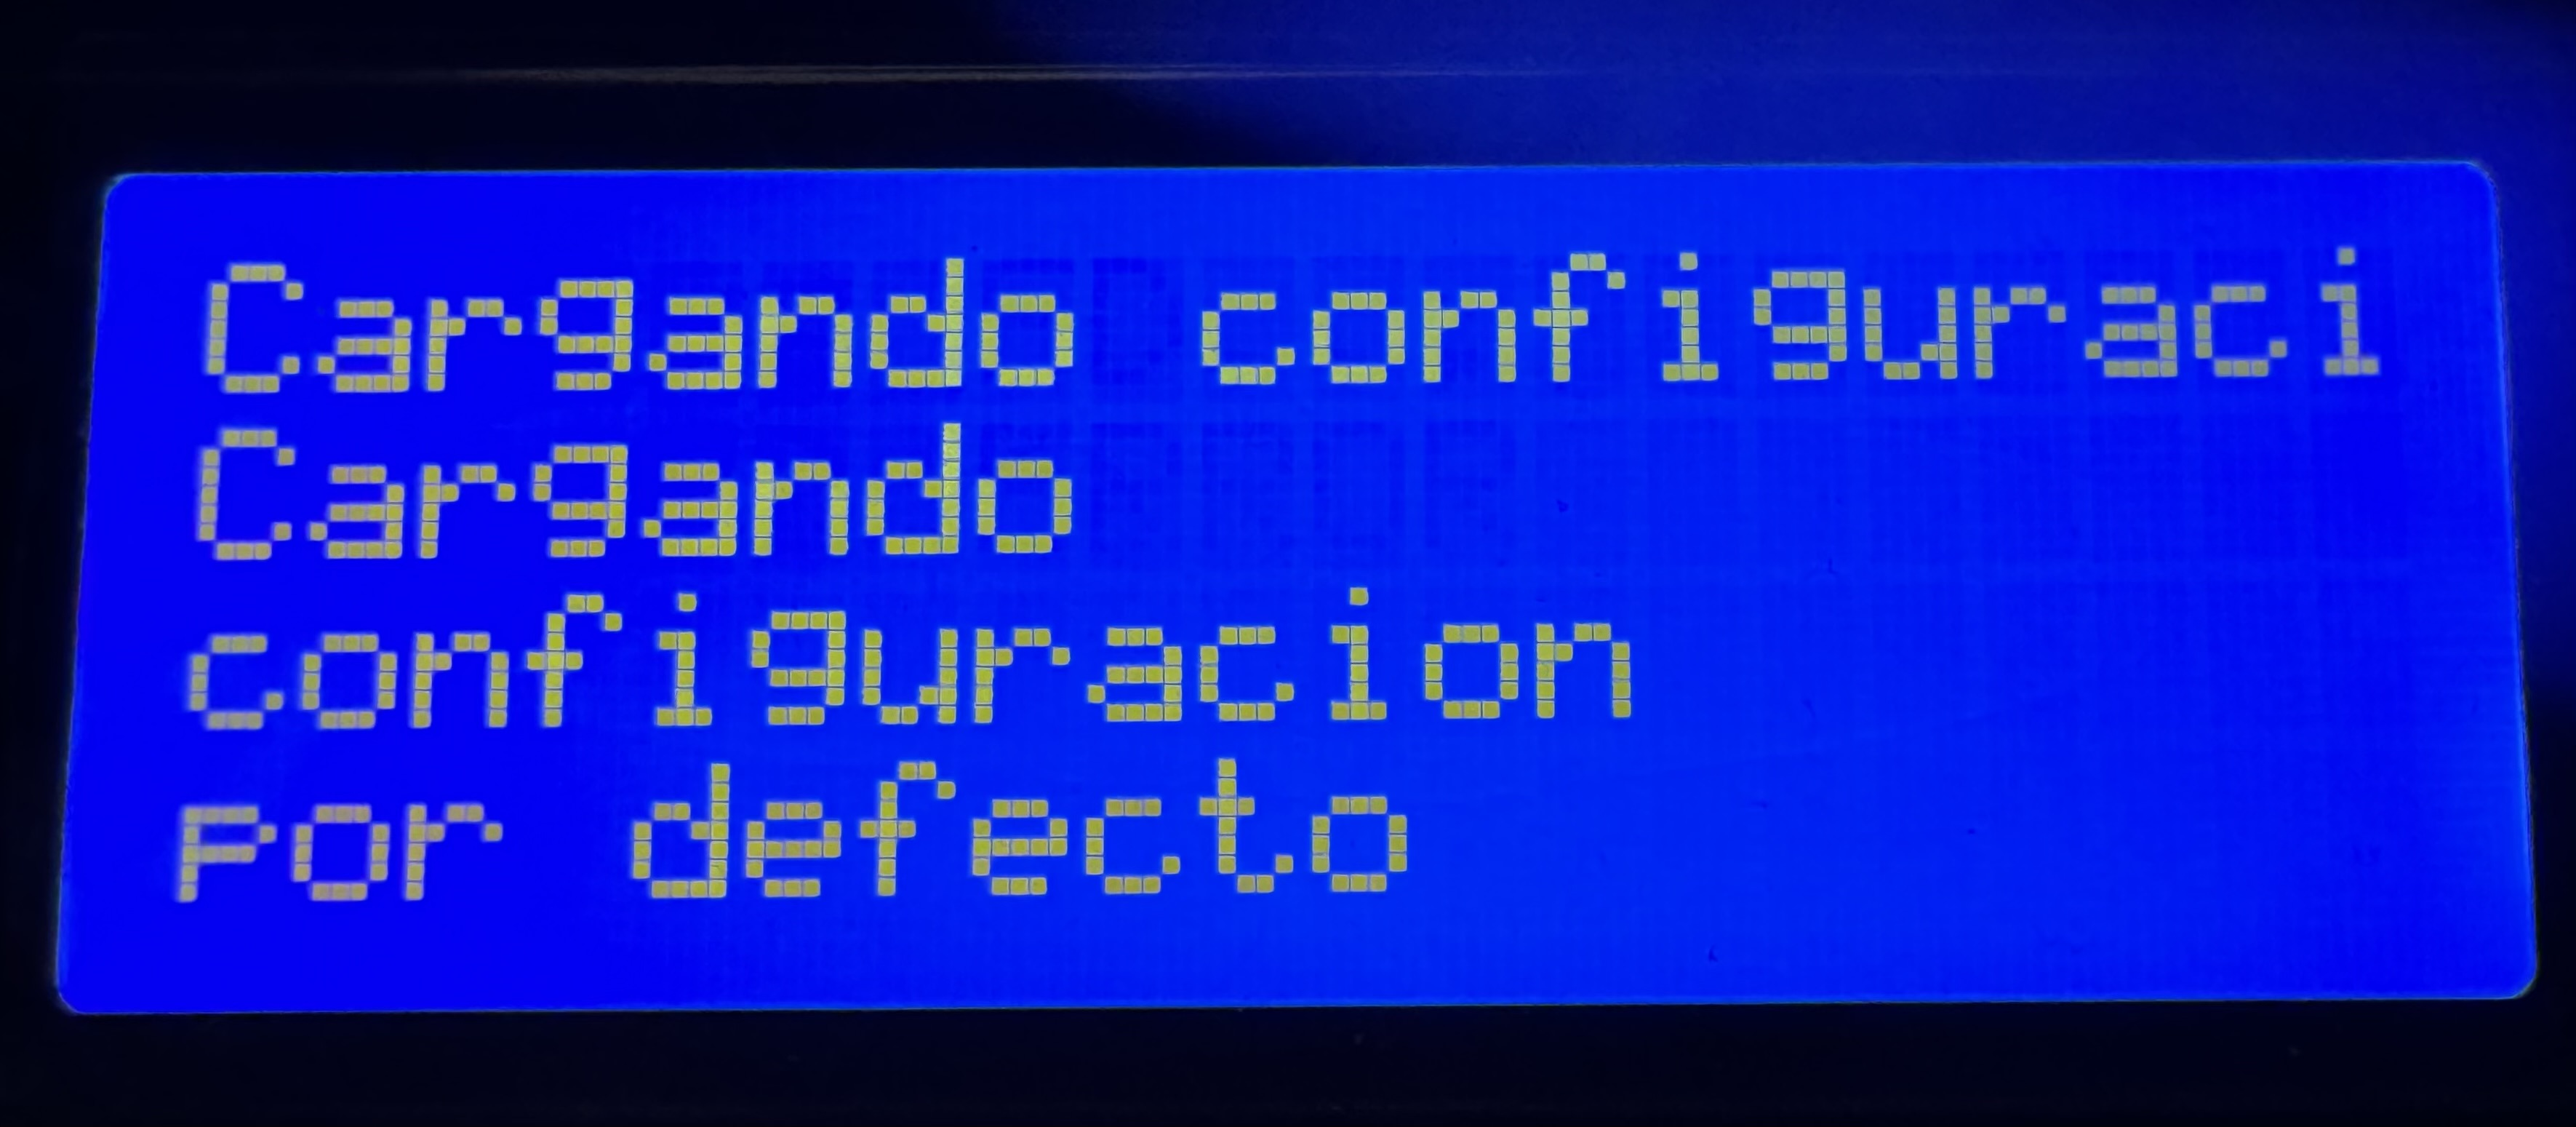
\psfig{file=Figuras/Conf_def.jpeg,width=8cm,angle=0}} 
\caption{Cargada configuración por defecto}\label{patalla:condef} 
\end{figure}

Que es la configuración aquí en Sevilla.

Puede ser interesante continuar si no existe el fichero \emph{config.txt}, porque al guardar cualquier configuración de cualquier sensor se creará el archivo en al tarjeta y podremos editarlo para poner la configuración WIFI a posteriori.

%%%%%%%%%%%%%%%%%%%%%%%%%%%%%%%%%%%%%%%%%%%%%%%%%%%%%%%%%%%%%%%%%%%%%%%%%%%%%%%%%%%%%%%%%%%%%

\item En caso de que la tarjeta microSd esté bien configurada (figura \ref{patalla:sd}). 

\begin{figure}[htbp!] 
\centering{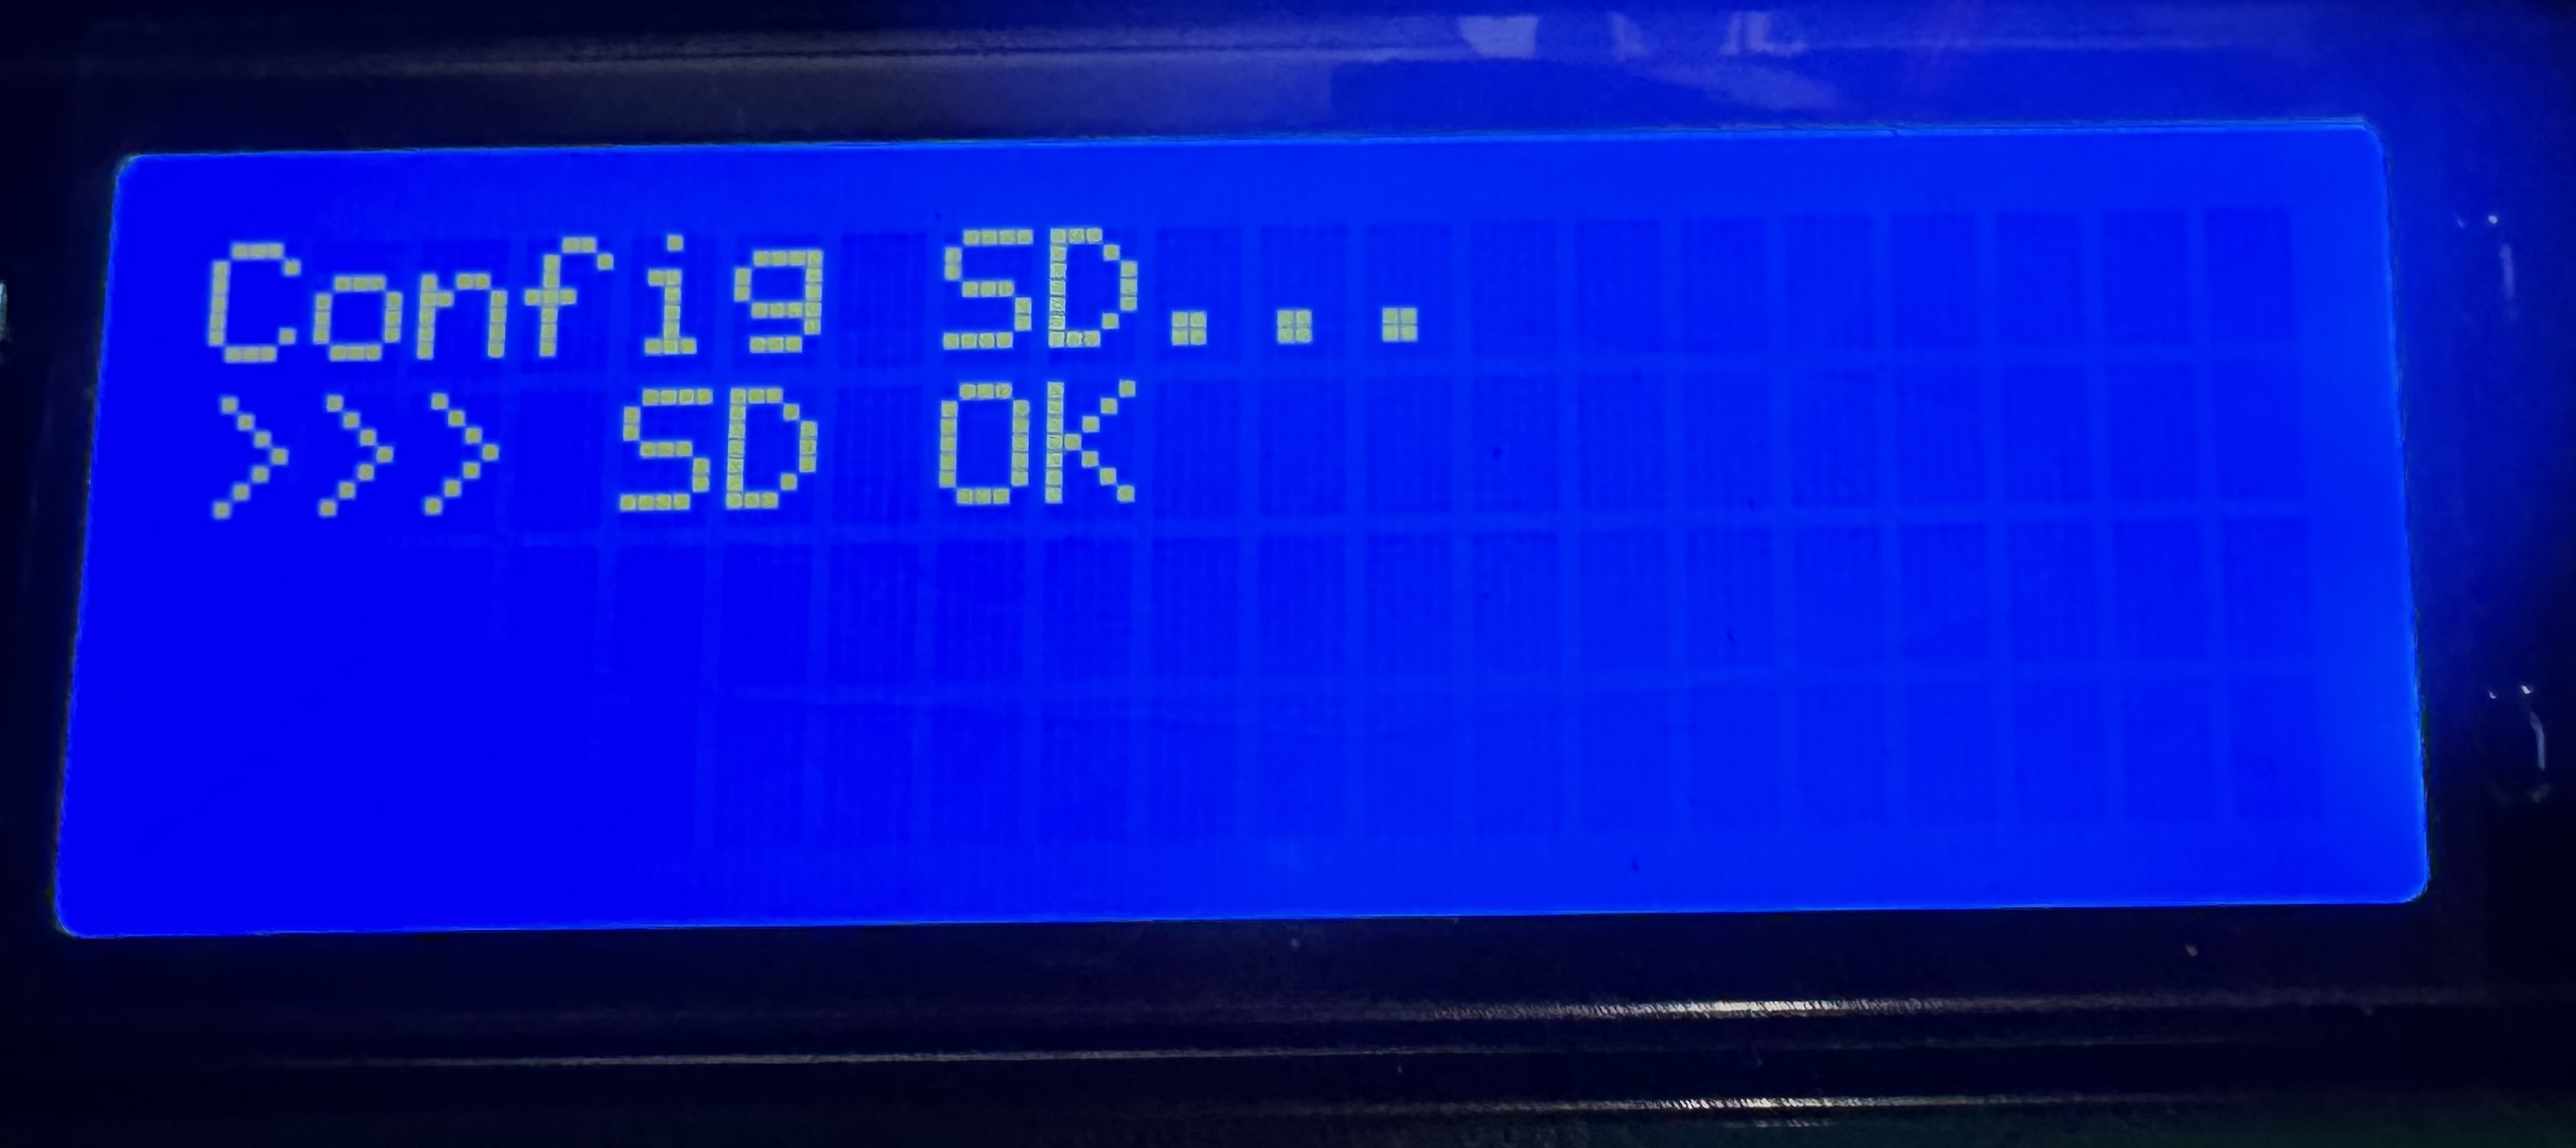
\psfig{file=Figuras/SD_OK.jpeg,width=8cm,angle=0}} 
\caption{SD OK}\label{patalla:sd} 
\end{figure}

Carga la configuración de los sensores (figura \ref{patalla:SenOk}).

\begin{figure}[htbp!] 
\centering{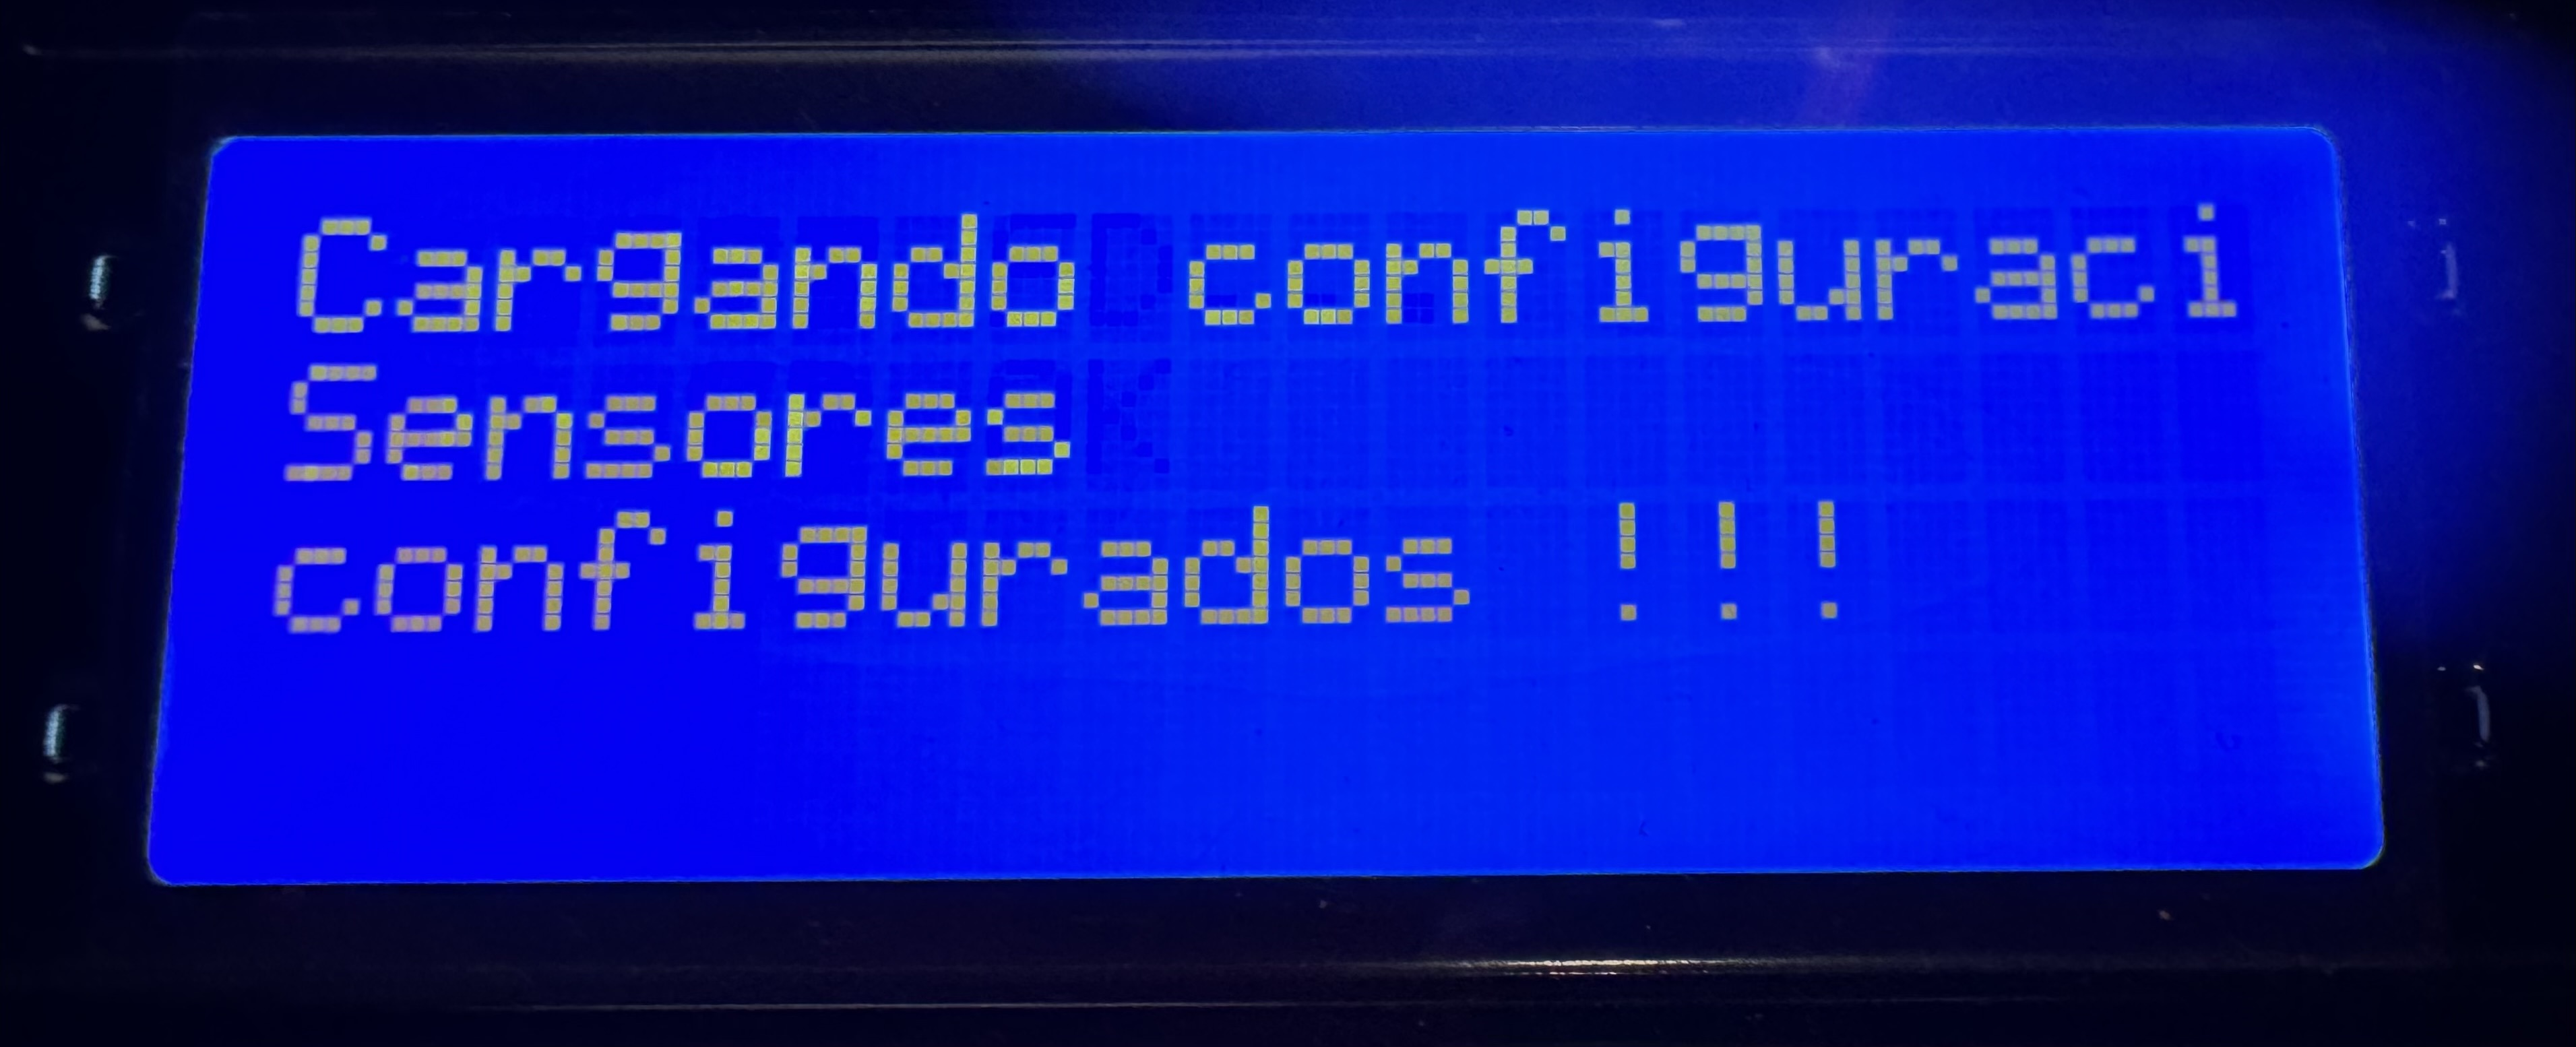
\psfig{file=Figuras/sensores_OK.jpeg,width=8cm,angle=0}} 
\caption{Cargada la configuración de los sensores}\label{patalla:SenOk} 
\end{figure}

%%%%%%%%%%%%%%%%%%%%%%%%%%%%%%%%%%%%%%%%%%%%%%%%%%%%%%%%%%%%%%%%%%%%%%%%%%%%%%%%%%%%%%%%%%%%%%%%
\newpage
\item Después configura la WIFI. Lo intentará 5 veces y si con ninguna de los 5 lo consigue aparecerá por pantalla:

\begin{figure}[htbp!] 
\centering{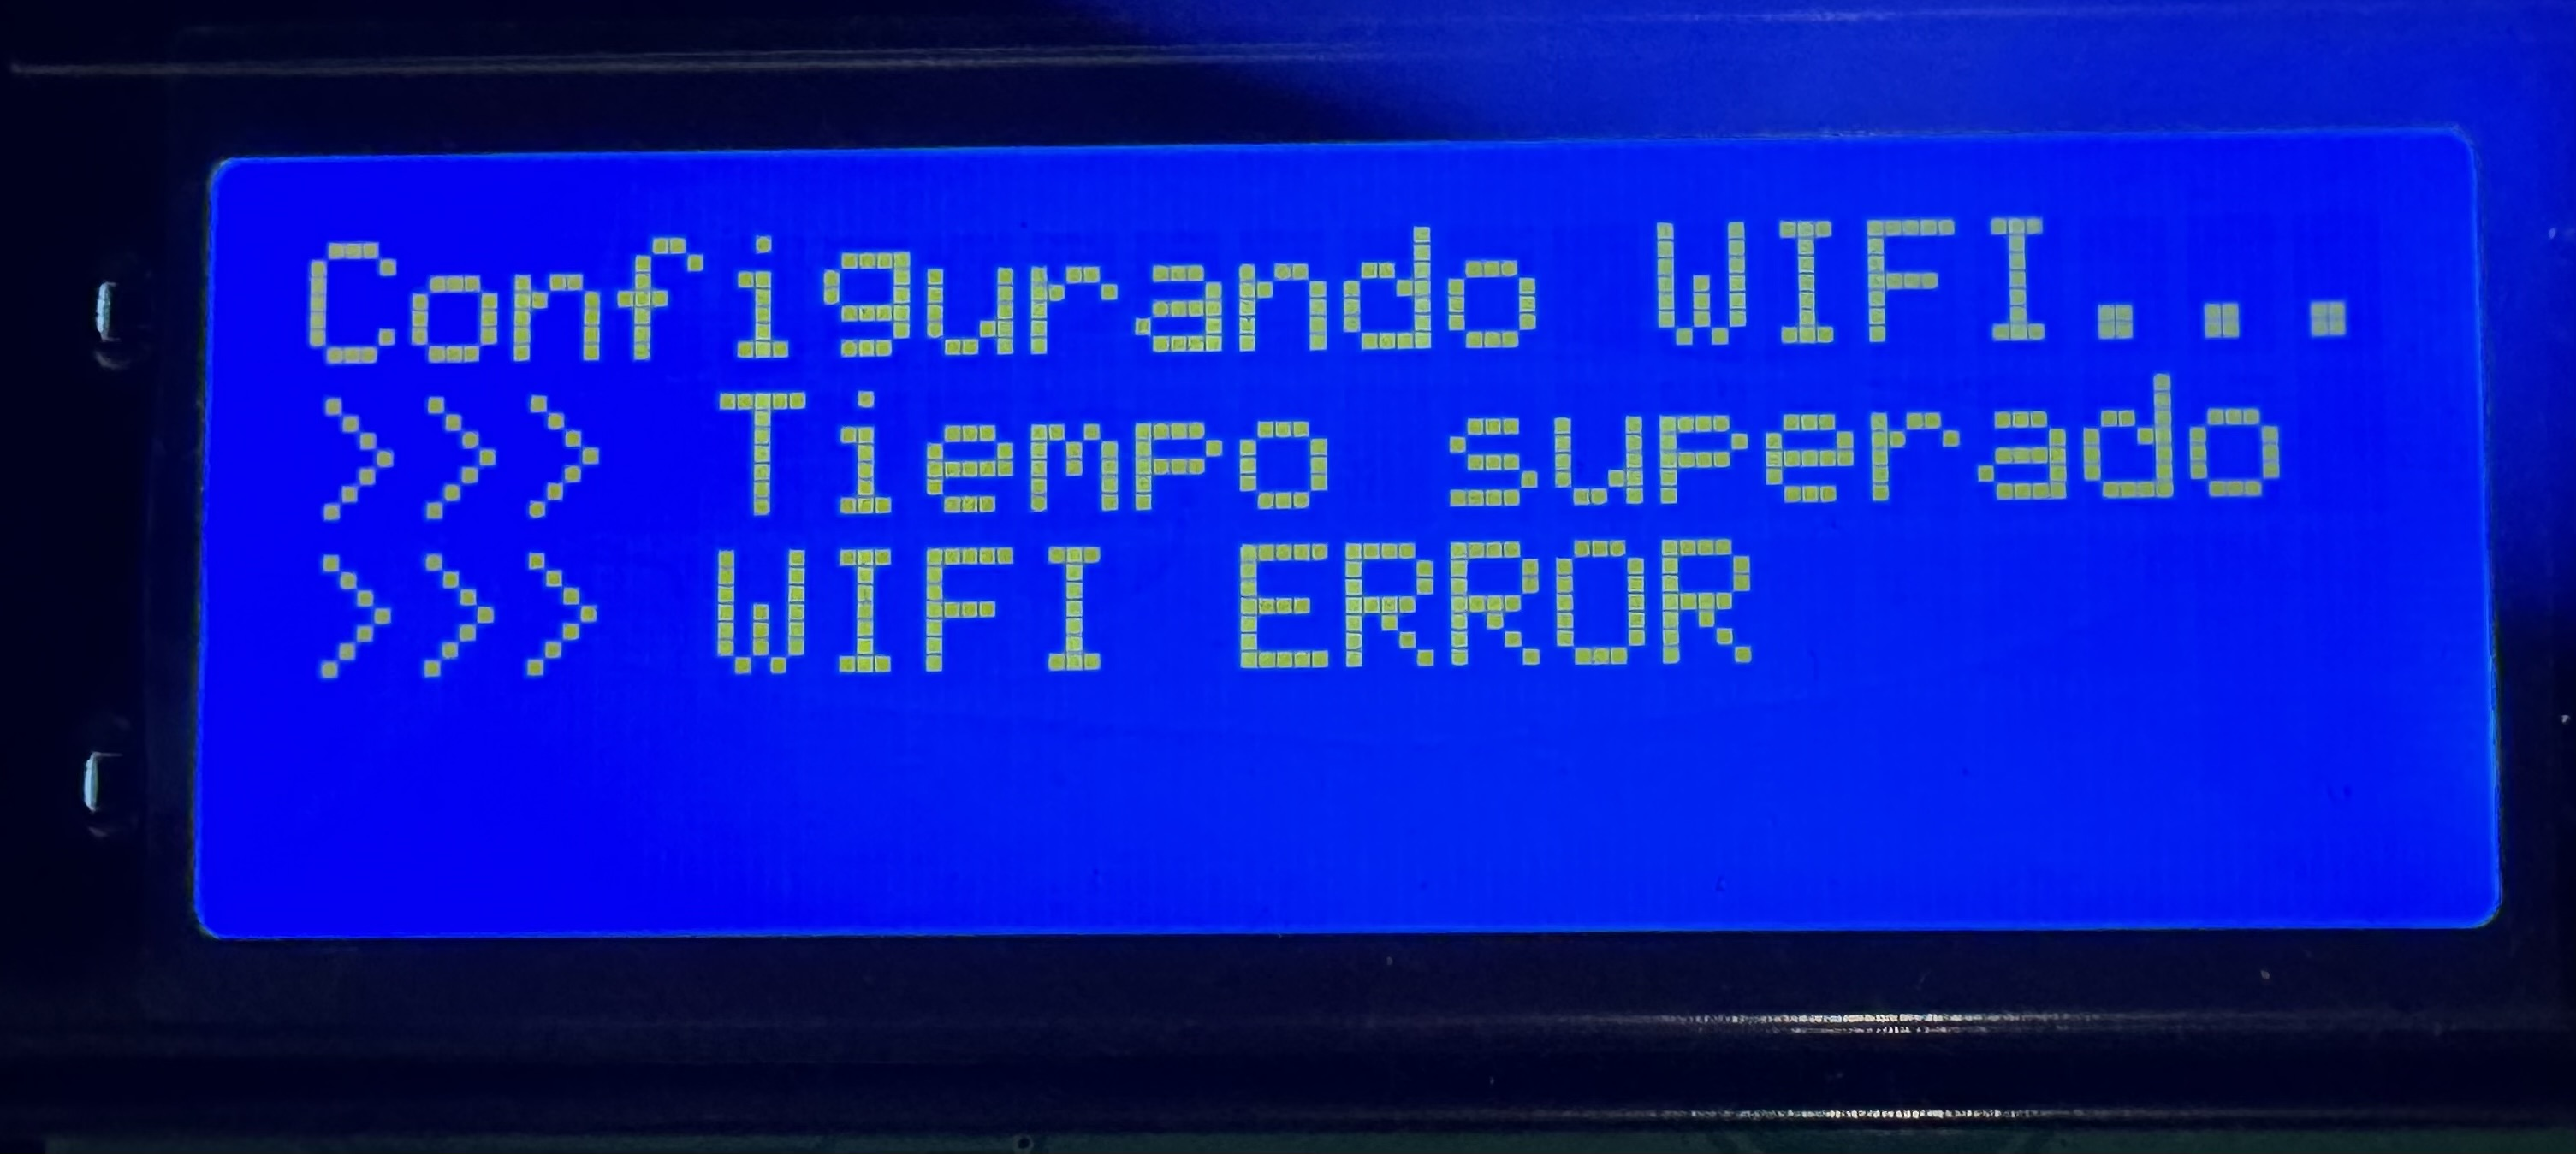
\psfig{file=Figuras/WIFI_ERROR.jpeg,width=8cm,angle=0}} 
\caption{No se ha podido conectar con la red WIFI}\label{patalla:wifiError} 
\end{figure}

Lo volverá a intentar 5 cada vez que quiera mandar un dato.

Si se consigue realizar la conexión con la WIFI aparecerá por pantalla el mensaje (figura \ref{patalla:WifiOk})

\begin{figure}[htbp!] 
\centering{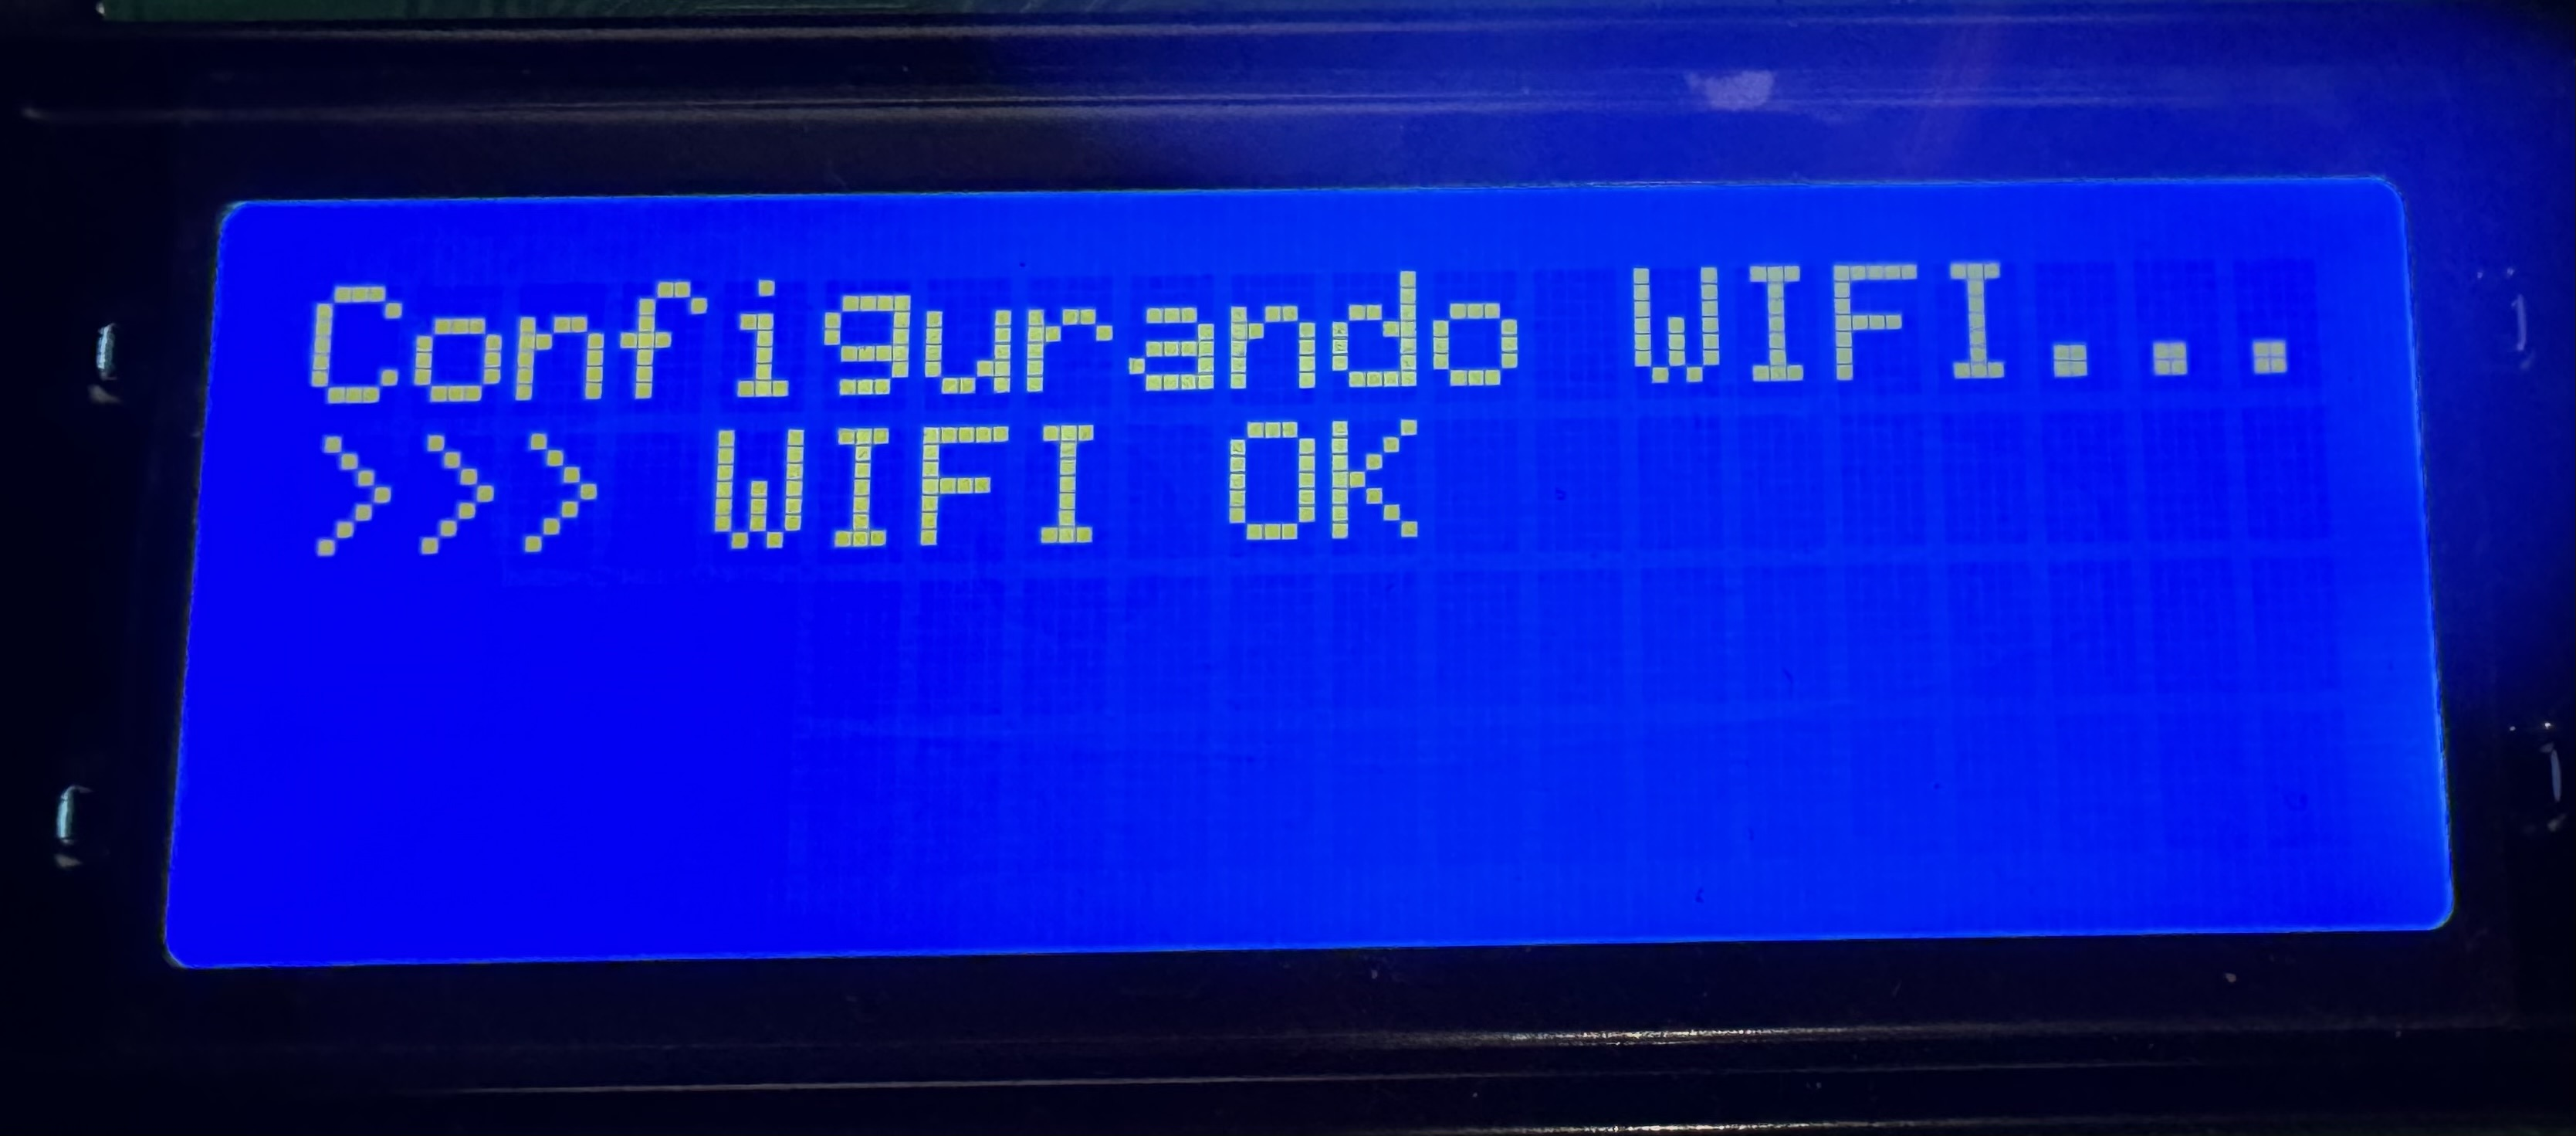
\psfig{file=Figuras/WIFI_OK.jpeg,width=8cm,angle=0}} 
\caption{Cargada la configuración de los sensores}\label{patalla:WifiOk} 
\end{figure}

Se encenderá el led con la etiqueta WIFI de la figura \ref{botones}.

%%%%%%%%%%%%%%%%%%%%%%%%%%%%%%%%%%%%%%%%%%%%%%%%%%%%%%%%%%%%%%%%%%%%%%%%%%%%%%%%%%%%%%%%%%%%%%%%

\item Si se ha podido configurar la WIFI, actualizará la hora interna del módulo de reloj. La actualiza con la hora GMT0 y luego se corregirá en función de donde se encuentre la instalación (figura \ref{patalla:relojOK})

\begin{figure}[htbp!] 
\centering{\psfig{file=Figuras/reloj_OK.jpeg,width=8cm,angle=0}} 
\caption{Módulo de reloj actualizado}\label{patalla:relojOK} 
\end{figure}


%%%%%%%%%%%%%%%%%%%%%%%%%%%%%%%%%%%%%%%%%%%%%%%%%%%%%%%%%%%%%%%%%%%%%%%%%%%%%%%%%%%%%%%%%%%%%%%%

\item A continuación intentará conectarse con el servidor mqtt. Si la WIFI está OK no habrá problemas a no ser que el servidor de Ayesa esté caído. Si no se puede aparecerá la siguiente pantalla (figura \ref{patalla:mqttError})

\begin{figure}[htbp!] 
\centering{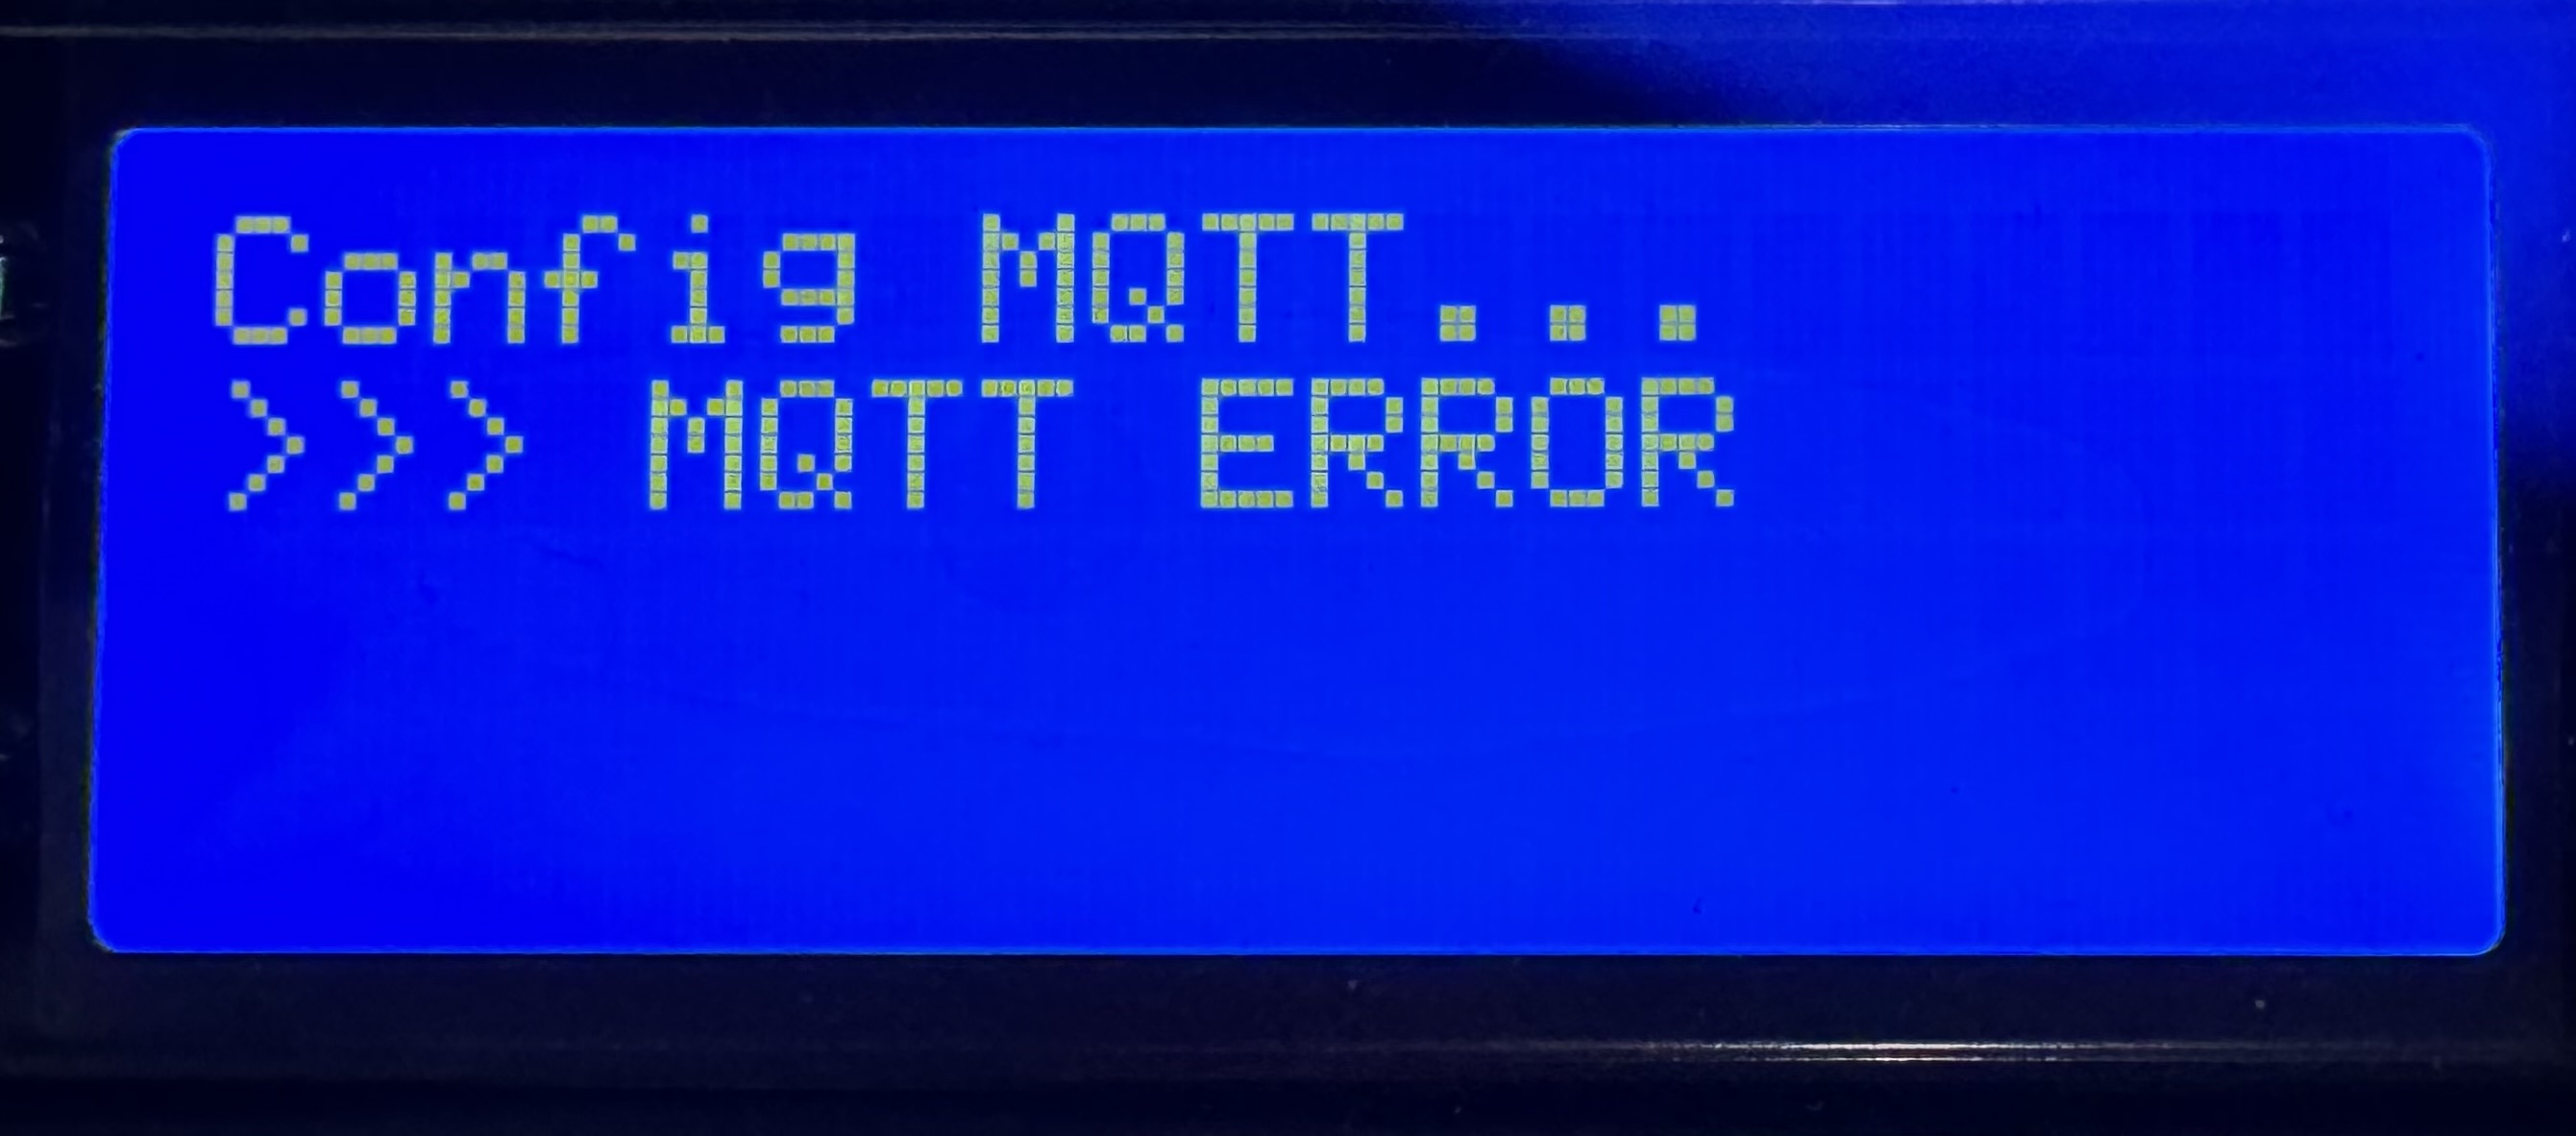
\psfig{file=Figuras/mqtt_ERROR.jpeg,width=8cm,angle=0}} 
\caption{Error al conectarse al sevidor mqtt}\label{patalla:mqttError} 
\end{figure}

Esta tarea requiere cierto tiempo porque lo intentará 5 veces. Durante el funcionamiento normal del dispositivo, cada vez que intente mandar un dato, chequeará el servidor MQTT y si no hay conexión, volverá a intentar conectarse 5 veces.

En caso de que que se conecte, aparecerá pantalla (figura \ref{patalla:mqttOK}). Además se encenderá el led con la etiqueta \emph{MQTT} de la figura \ref{botones}.

\begin{figure}[htbp!] 
\centering{\psfig{file=Figuras/mqtt_OK.jpeg,width=8cm,angle=0}} 
\caption{Éxito al conectarse al sevidor mqtt}\label{patalla:mqttOK} 
\end{figure}

%%%%%%%%%%%%%%%%%%%%%%%%%%%%%%%%%%%%%%%%%%%%%%%%%%%%%%%%%%%%%%%%%%%%%%%%%%%%%%%%%%%%%%%%%%%%%%%%

\item A continuación entra en el modo de funcionamiento normal, donde aparecerán dos pantallas que alternan cada 5 segundos. La primera muestra las variables relacionadas con el agua y la segunda con el aire.

En la pantalla\footnote{Los valores que aparecen en la pantalla no son reales pues cuando se hizo esta guía el dispositivo no tenía sensores conectados} relacionada con el agua puede verse (figura \ref{patalla:1}):
\begin{itemize}
\item Línea 1: hora y fecha
\item Línea 2: temperatura TW1 que es la temperatura de la sonda de conductividad. Y la temperatura TW2 es la temperatura proporcionada por el sensor DS18B20.
\item Línea 3: Valor de la conductividad
\item Línea 4: valor del PH y de la concentración de $O_2$
\end{itemize}

\begin{figure}[htbp!] 
\centering{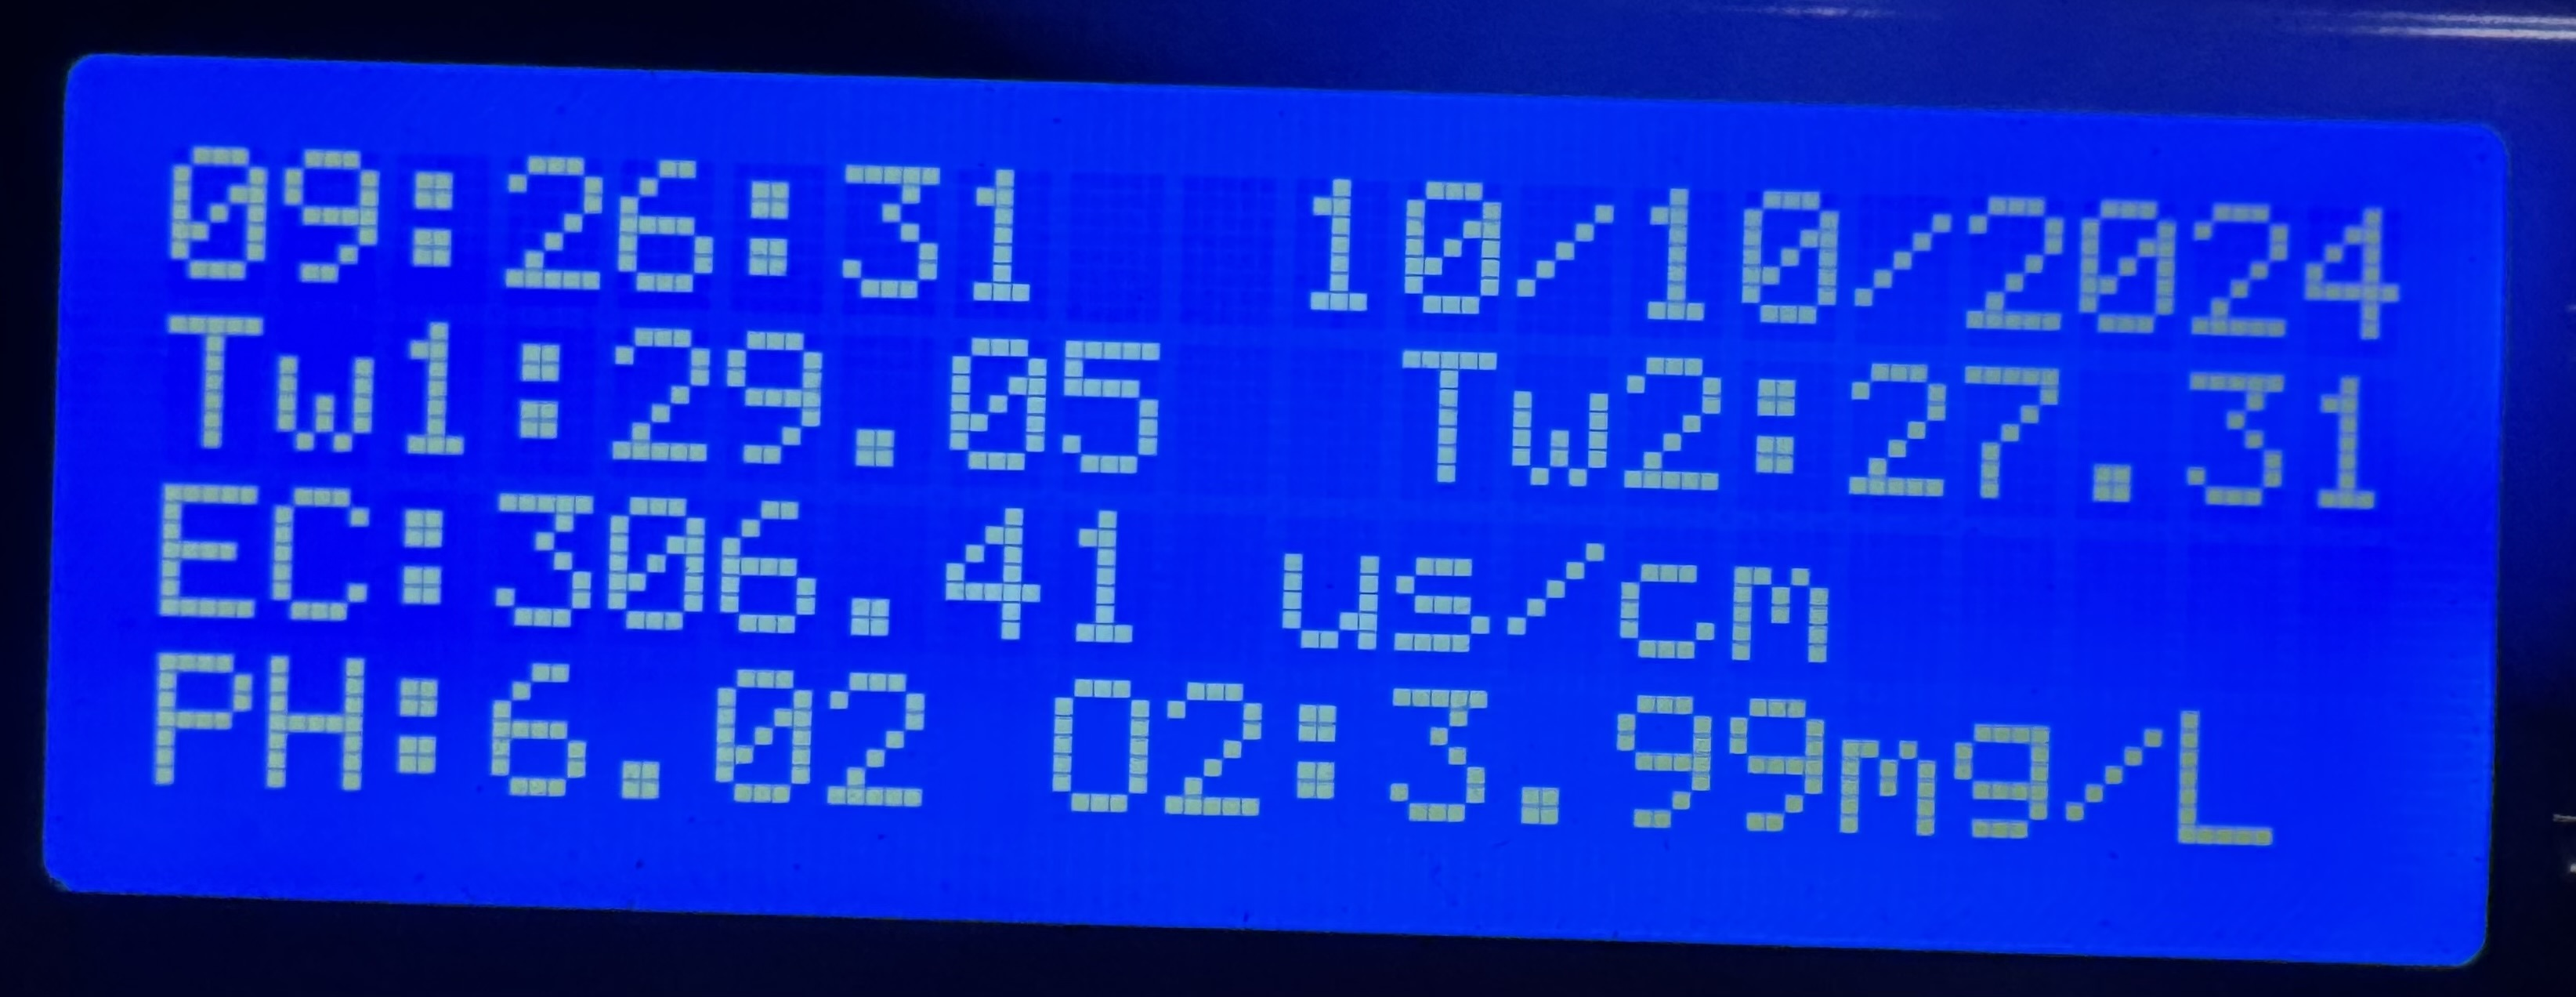
\psfig{file=Figuras/pantalla1.jpeg,width=8cm,angle=0}} 
\caption{Pantalla que muestra las variables relacionadas con el agua}\label{patalla:1} 
\end{figure}

En la pantalla relacionada con el agua puede verse (figura \ref{patalla:2}):
\begin{itemize}
\item Línea 1: hora y fecha
\item Línea 2: VAR AMB, para recordar que son variables ambientales.
\item Línea 3: Valores de temperatura y humedad del aire del sensor DTH22 conectado en el puerto de la placa DTH22A.
\item Línea 4: Valores de temperatura y humedad del aire del sensor DTH22 conectado en el puerto de la placa DTH22B.
\end{itemize}

\begin{figure}[htbp!] 
\centering{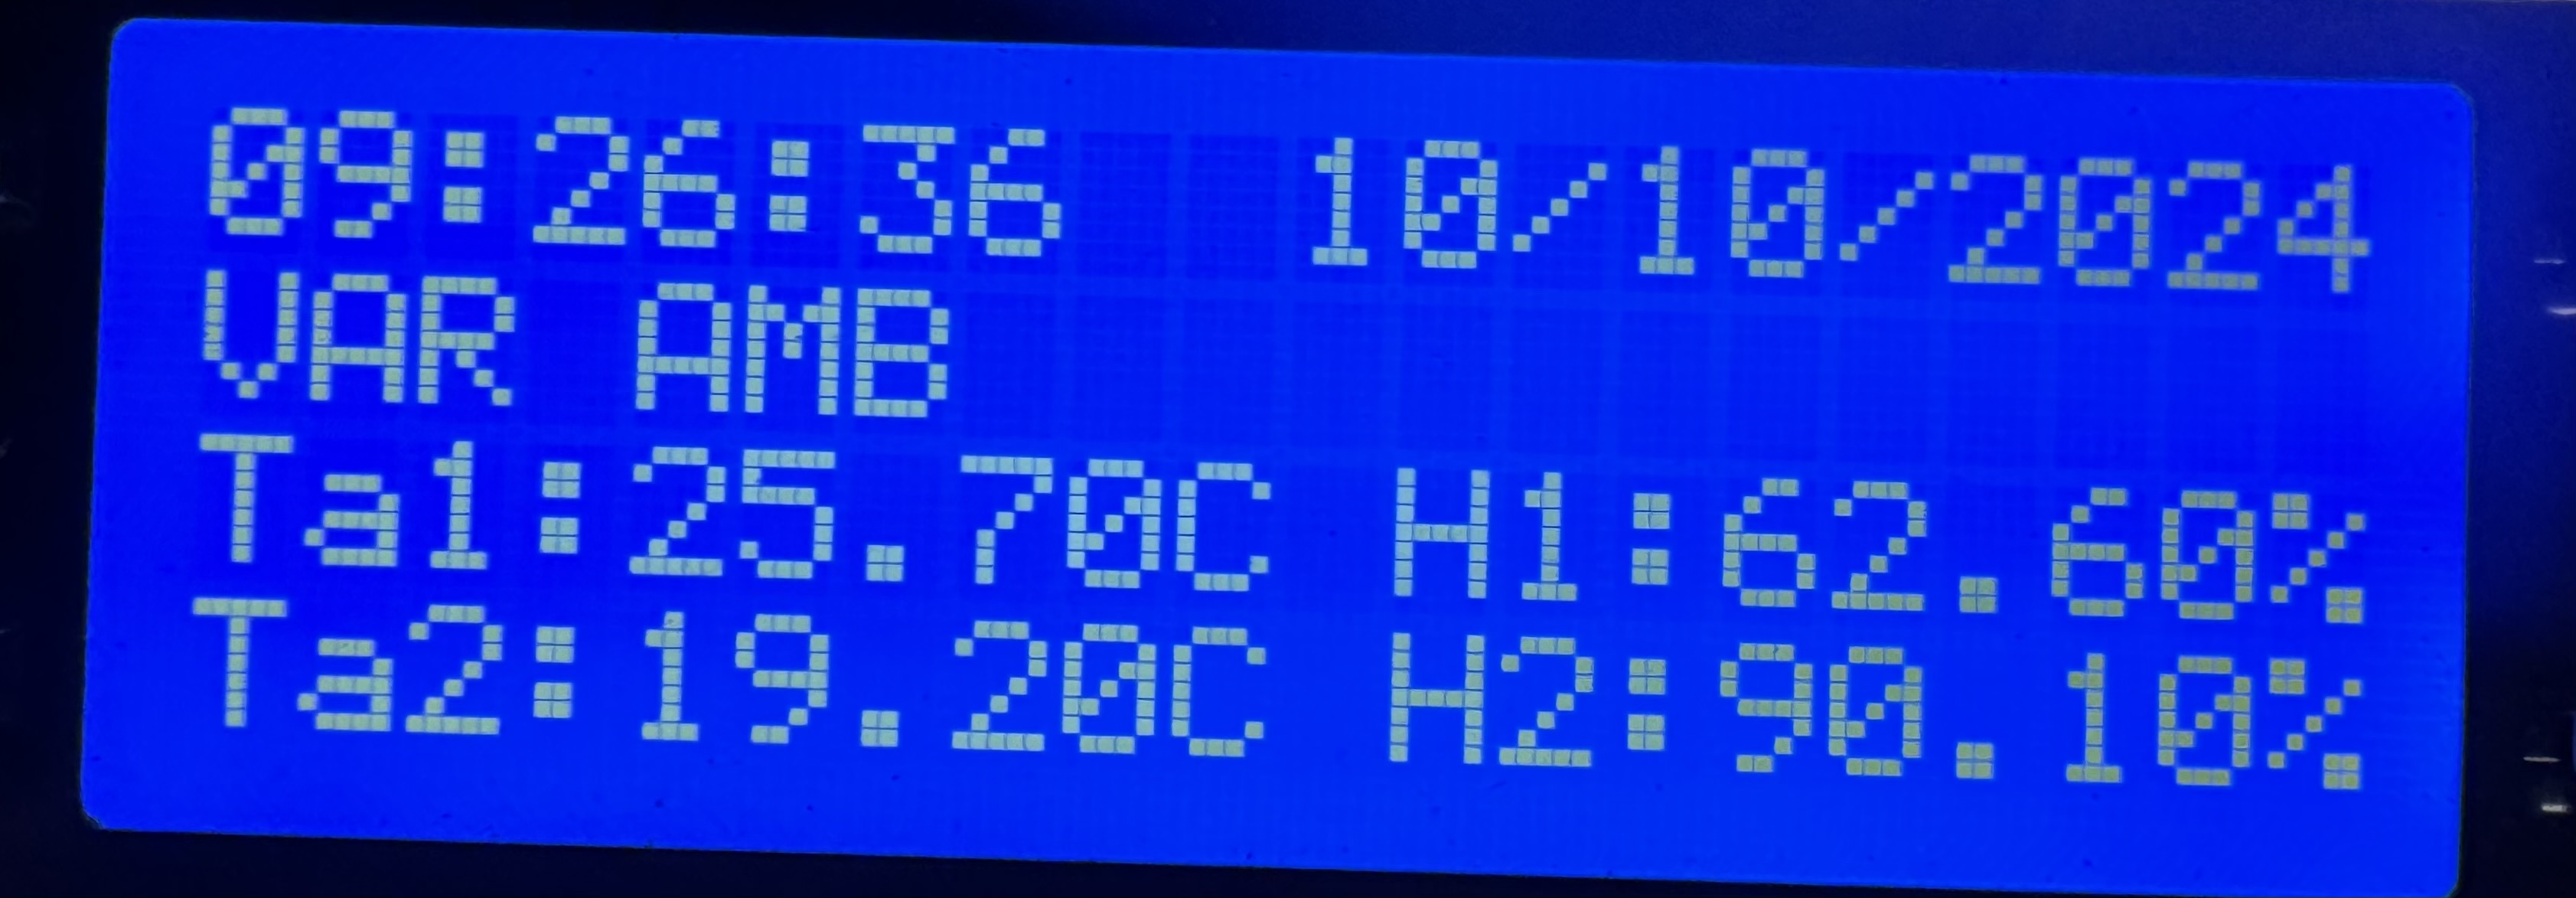
\psfig{file=Figuras/pantalla2.jpeg,width=8cm,angle=0}} 
\caption{Pantalla que muestra las variables relacionadas con el aire}\label{patalla:2} 
\end{figure}

\end{enumerate}

%%%%%%%%%%%%%%%%%%%%%%%%%%%%%%%%%%%%%%%%%%%%%%%%%%%%%%%%%%%%%%%%%%%%%%%%%%%%%%%%%%%%%%%%%%%%%%%%
\newpage
\section{Sensor de PH y calibración}

El sensor que se usa en este proyecto es un DFRobot SEN0169-V2 en su versión con probeta industrial:
\begin{verbatim}
https://www.dfrobot.com/product-2069.html
https://wiki.dfrobot.com/Gravity__Analog_pH_Sensor_Meter_Kit_V2_SKU_SEN0161-V2
\end{verbatim}
El medidor de pH analógico por gravedad V2 de DFRobot está diseñado específicamente para medir el pH de una solución y reflejar su acidez o alcalinidad. La señal de salida se filtra por hardware y tiene una fluctuación general baja.

El sensor de PH nos dará una tensión que va de 0V a 3V. El fabricante dice que el PH y la tensión tiene una relación lineal por lo que con tener dos punto de esa recta sería suficiente para poder calibrar dicho sensor. 
\subsection{Primer punto de la recta de PH}

Una vez estamos en la pantalla principal pulsamos el botón MODE una única vez\footnote{Si se pasa la pantalla, siga pulsando hasta que vuelva la pantalla principal} hasta que sale la pantalla (figura \ref{patalla:PH1}). Fíjese que es la parte superior aparece la frase: \textbf{CAL PH1}.

\begin{figure}[htbp!] 
\centering{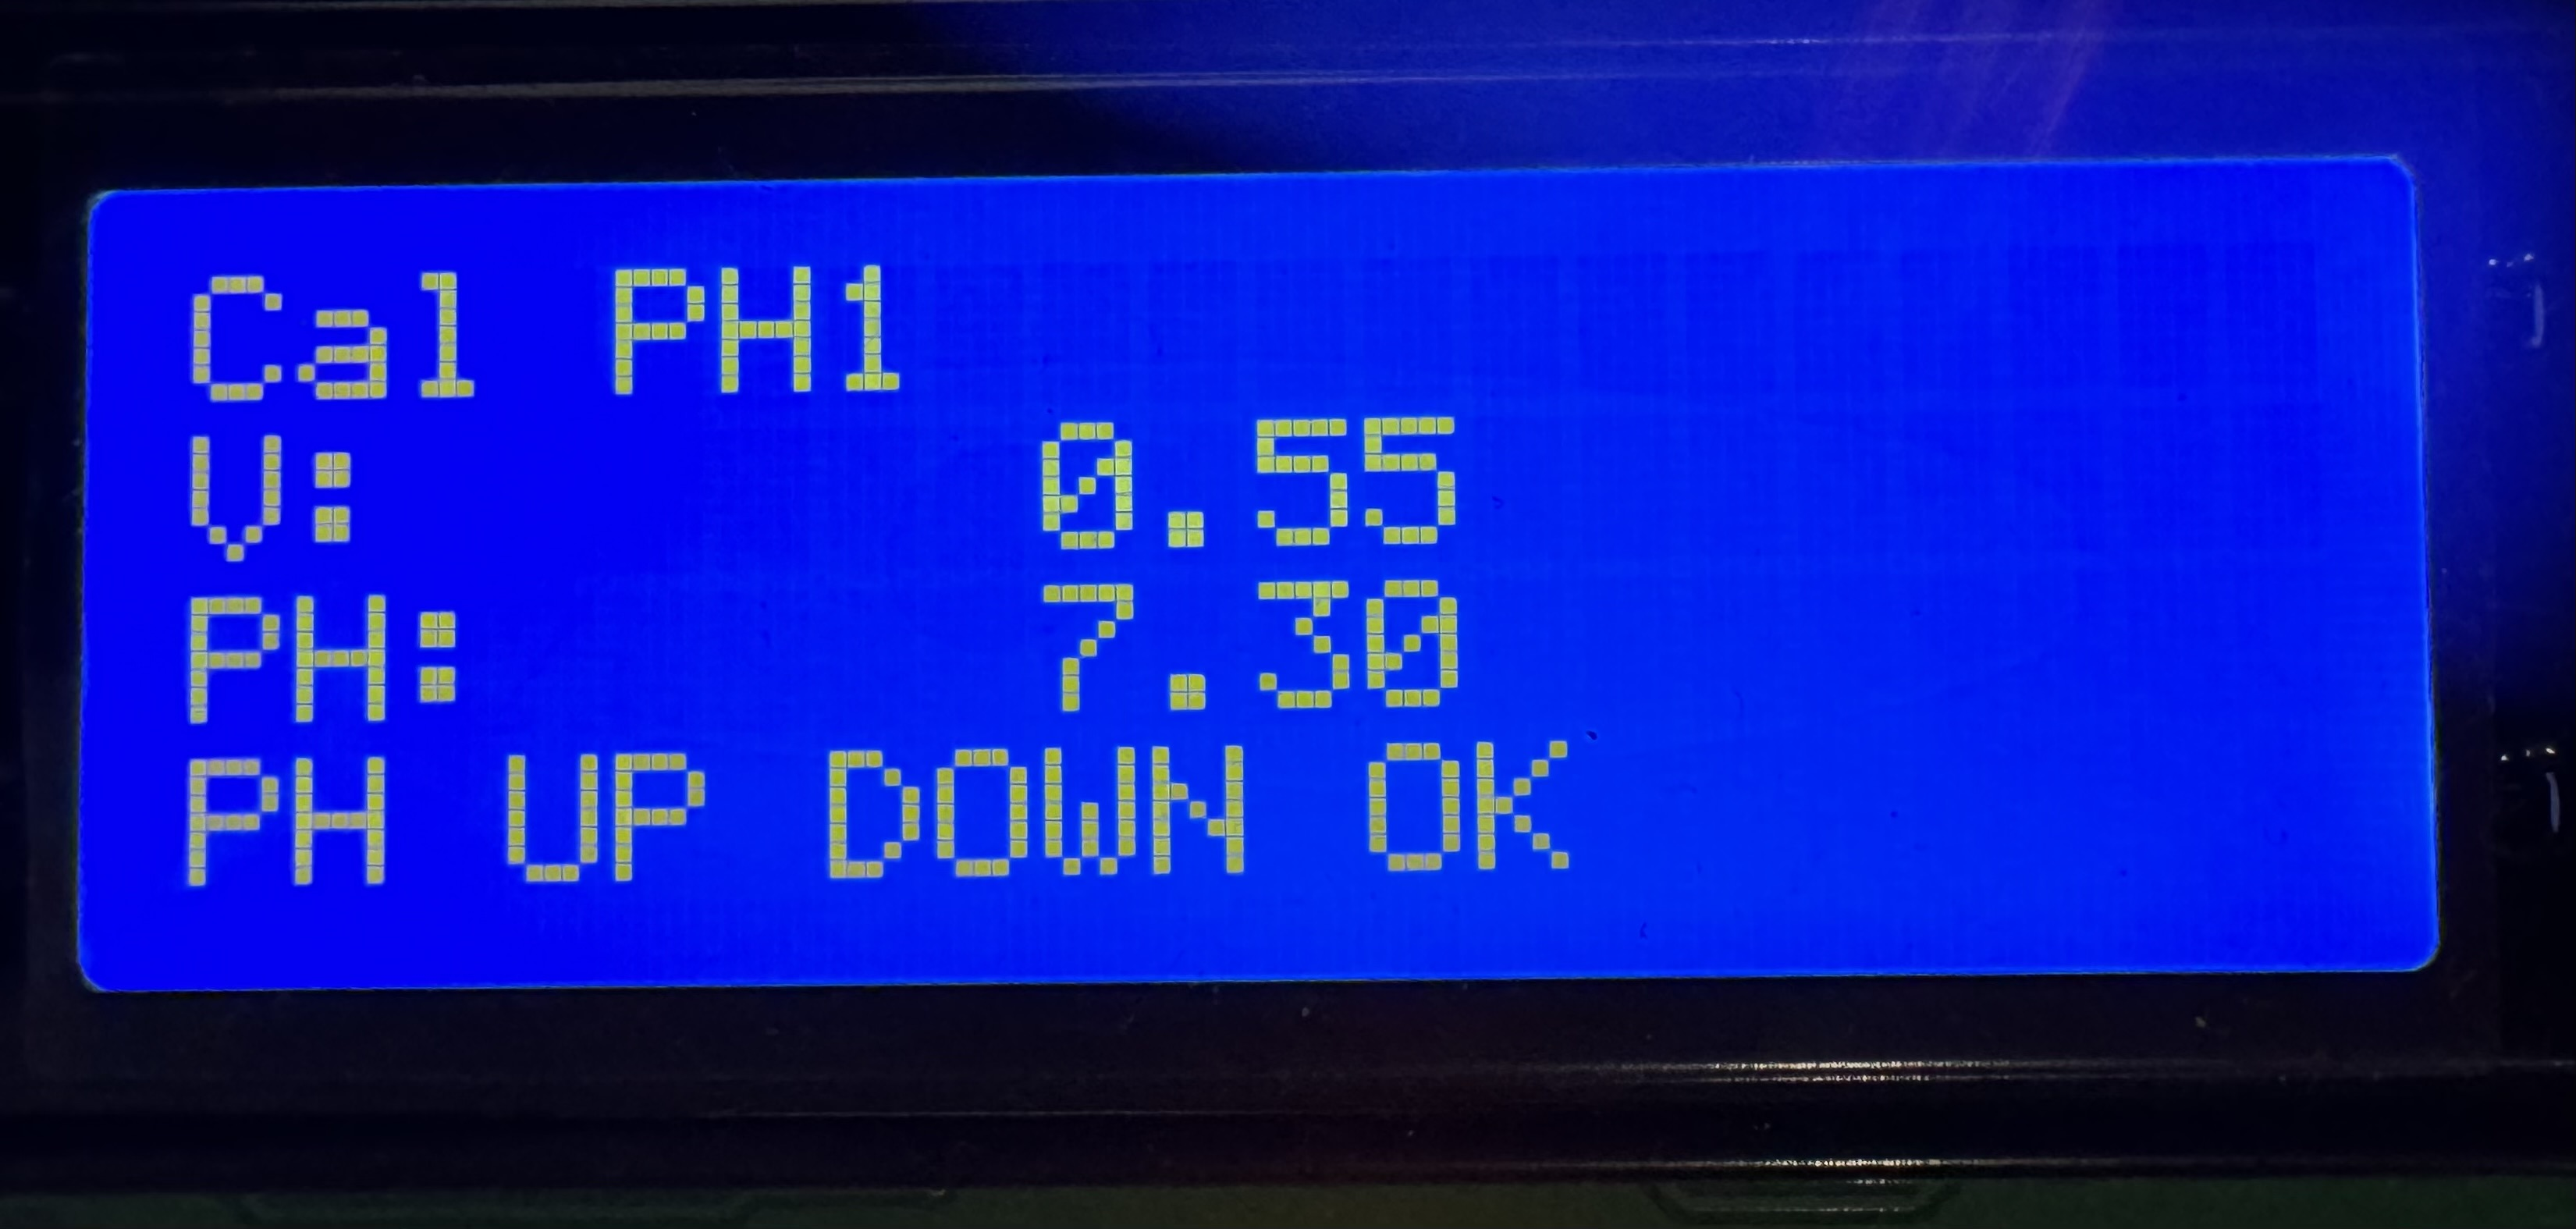
\psfig{file=Figuras/PH1.jpeg,width=8cm,angle=0}} 
\caption{Primer punto de calibración del sensor de PH}\label{patalla:PH1} 
\end{figure}

\begin{itemize}
\item Línea 1: \textbf{CAL PH1}.
\item Línea 2: \textbf{V:} es la tensión que está leyendo el sensor.
\item Línea 3: \textbf{PH:}Valor de PH de ese punto (lo establecemos pulsando UP o DOWN para incrementar o decrementar dicho valor 0.1. 
\item Línea 4: \textbf{PH UP DOWN OK}. Podemos variar el PH con UP o DOWN y una vez que este todo pulsamos OK para acabar.
\end{itemize}

El procedimiento es el siguiente: Metemos la probeta del PH previa limpieza en un líquido de PH conocido y \underline{esperamos un minuto} a que se estabilice la tensión. Ajustamos el campo PH con UP y DOWN y pulsamos OK. En ese momento se ajusta el primer punto de la recta característica del sensor de PH. 

En el archivo \emph{config.txt} se actualizaran los valores \emph{PH1} y \emph{mV1}.

\subsection{Segundo punto de la recta de PH}

Una vez estamos en la pantalla principal pulsamos el botón MODE dos veces\footnote{Si se pasa la pantalla, siga pulsando hasta que vuelva la pantalla principal} hasta que sale la pantalla (figura \ref{patalla:PH2}). Fíjese que es la parte superior aparece la frase: \textbf{CAL PH2}.

\begin{figure}[htbp!] 
\centering{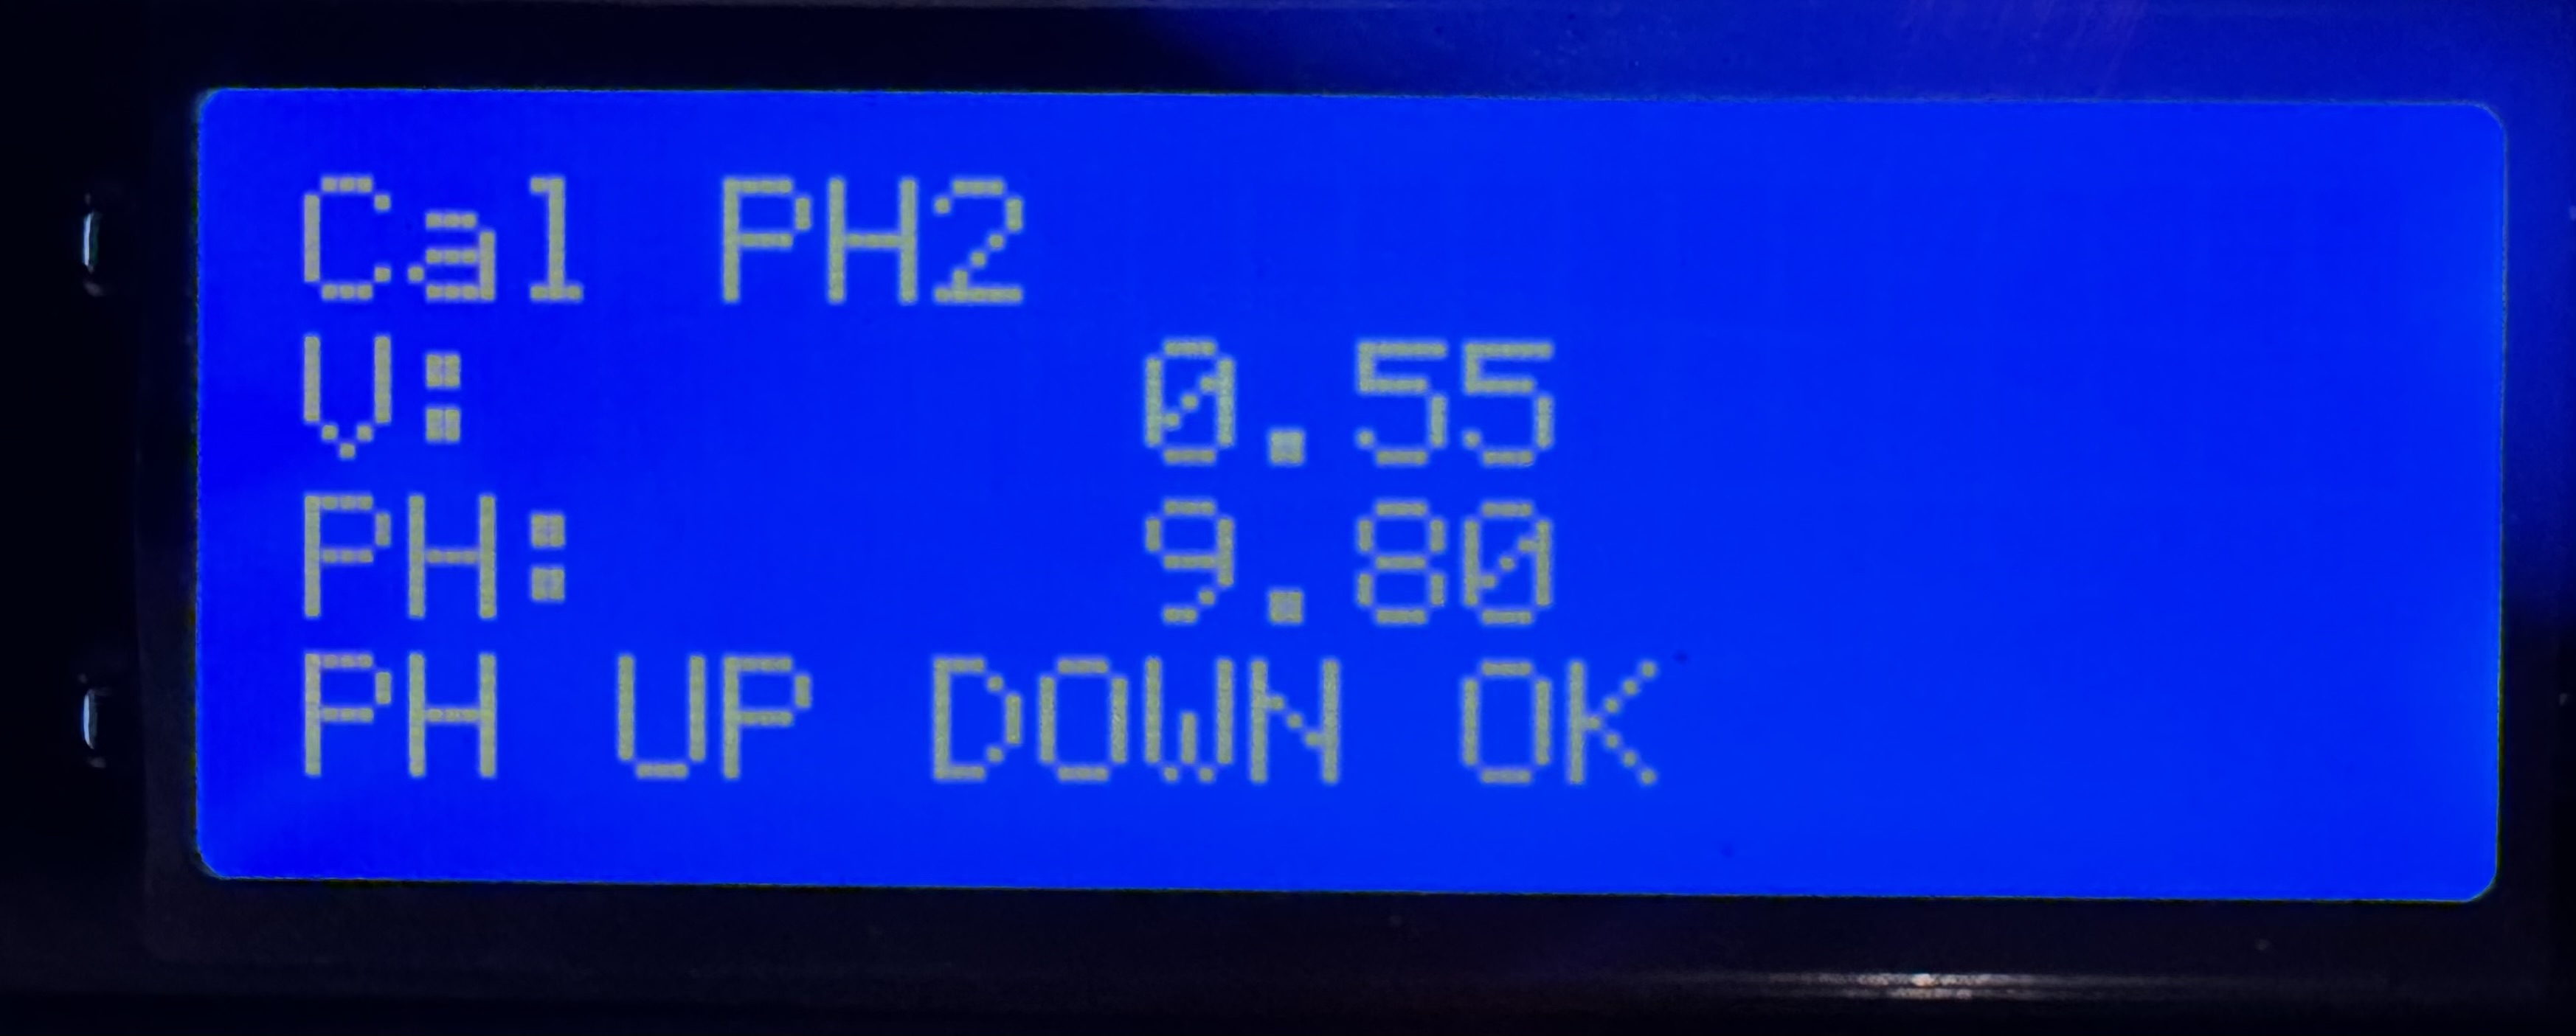
\psfig{file=Figuras/PH2.jpeg,width=8cm,angle=0}} 
\caption{Segundo punto de calibración del sensor de PH}\label{patalla:PH2} 
\end{figure}

\begin{itemize}
\item Línea 1: \textbf{CAL PH2}.
\item Línea 2: \textbf{V:} es la tensión que está leyendo el sensor.
\item Línea 3: \textbf{PH:}Valor de PH de ese punto (lo establecemos pulsando UP o DOWN para incrementar o decrementar dicho valor 0.1. 
\item Línea 4: \textbf{PH UP DOWN OK}. Podemos variar el PH con UP o DOWN y una vez que este todo pulsamos OK para acabar.
\end{itemize}

El procedimiento es el siguiente: Metemos la probeta del PH, previa limpieza, en el segundo líquido de PH conocido (con un  PH distinto del primero) y \underline{esperamos un minuto} a que se estabilice la tensión. Ajustamos el campo PH con UP y DOWN y pulsamos OK. En ese momento se ajusta el segundo punto de la recta característica del sensor de PH. 

En el archivo \emph{config.txt} se actualizaran los valores \emph{PH2} y \emph{mV2}.

\begin{tcolorbox}
[colback=red!5!white,colframe=red!75!black,fonttitle=\bfseries,title=CALIBRACIÓN SENSOR PH]
Este sensor se ha estado usando durante más de un año y como mejores resultados ha dado es:
\begin{enumerate}
\item Escogemos el primer punto de calibración un punto del PH típico, usando el propio baño de los peces como líquido de calibración. Medimos el PH con un sensor portátil y ajustamos el primer punto con dicho valor. Se chequea el valor del PH una vez al día y si hay desviación se corrige el punto 1 del sensor sobre la marcha.
\item El segundo punto hay que hacerlo con un PH ácido con una solución de PH conocido. la misma que se utiliza para calibrar el sensor de PH portátil. Este punto se recalibra una vez al mes como dice el fabricante.
\end{enumerate}
Según el fabricante la vida de la probeta es de 1 año. Mi experiencia es que haciendo frecuentes recalibraciones, la recta característica se va adaptando al deterioro de la sonda. Y dado que el PH no varía mucho se puede aguantar más tiempo.

\end{tcolorbox}




%%%%%%%%%%%%%%%%%%%%%%%%%%%%%%%%%%%%%%%%%%%%%%%%%%%%%%%%%%%%%%%%%%%%%%%%%%%%%%%%%%%%%%%%%%%%%%%%%%%%%%

\newpage
\section{Sensor de concentración de O2 y calibración}

El sensor que se usa en este proyecto es un DFRobot Sensor de oxigeno disuelto SEN0237-A. El sensor de oxígeno disuelto SEN0237-A es compatible con tarjetas Arduino. Se utiliza para medir la concentración de oxígeno en el agua. Este parámetro permite identificar la calidad del agua. Una baja concentración de oxígeno en el agua producirá una dificultad de respirar en organismos acuáticos. 
\begin{verbatim}
https://www.dfrobot.com/product-1628.html
https://wiki.dfrobot.com/Gravity__Analog_Dissolved_Oxygen_Sensor_SKU_SEN0237
\end{verbatim}

Hay tres procedimientos de calibración, pero para este proyecto solo se han programado dos de ellos:

\subsection{Procedimiento 1. Usando temperatura del aire}
Este es el procedimiento más sencillo y el que mejores resultados nos ha dado.
\begin{enumerate}
\item Una vez estamos en la pantalla principal pulsamos el botón MODE tres veces\footnote{Si se pasa la pantalla, siga pulsando hasta que vuelva la pantalla principal} hasta que sale la pantalla (figura \ref{patalla:O2aire}). Fíjese que es la parte superior aparece la frase: \textbf{Cal 02 T aire}.

\begin{figure}[htbp!] 
\centering{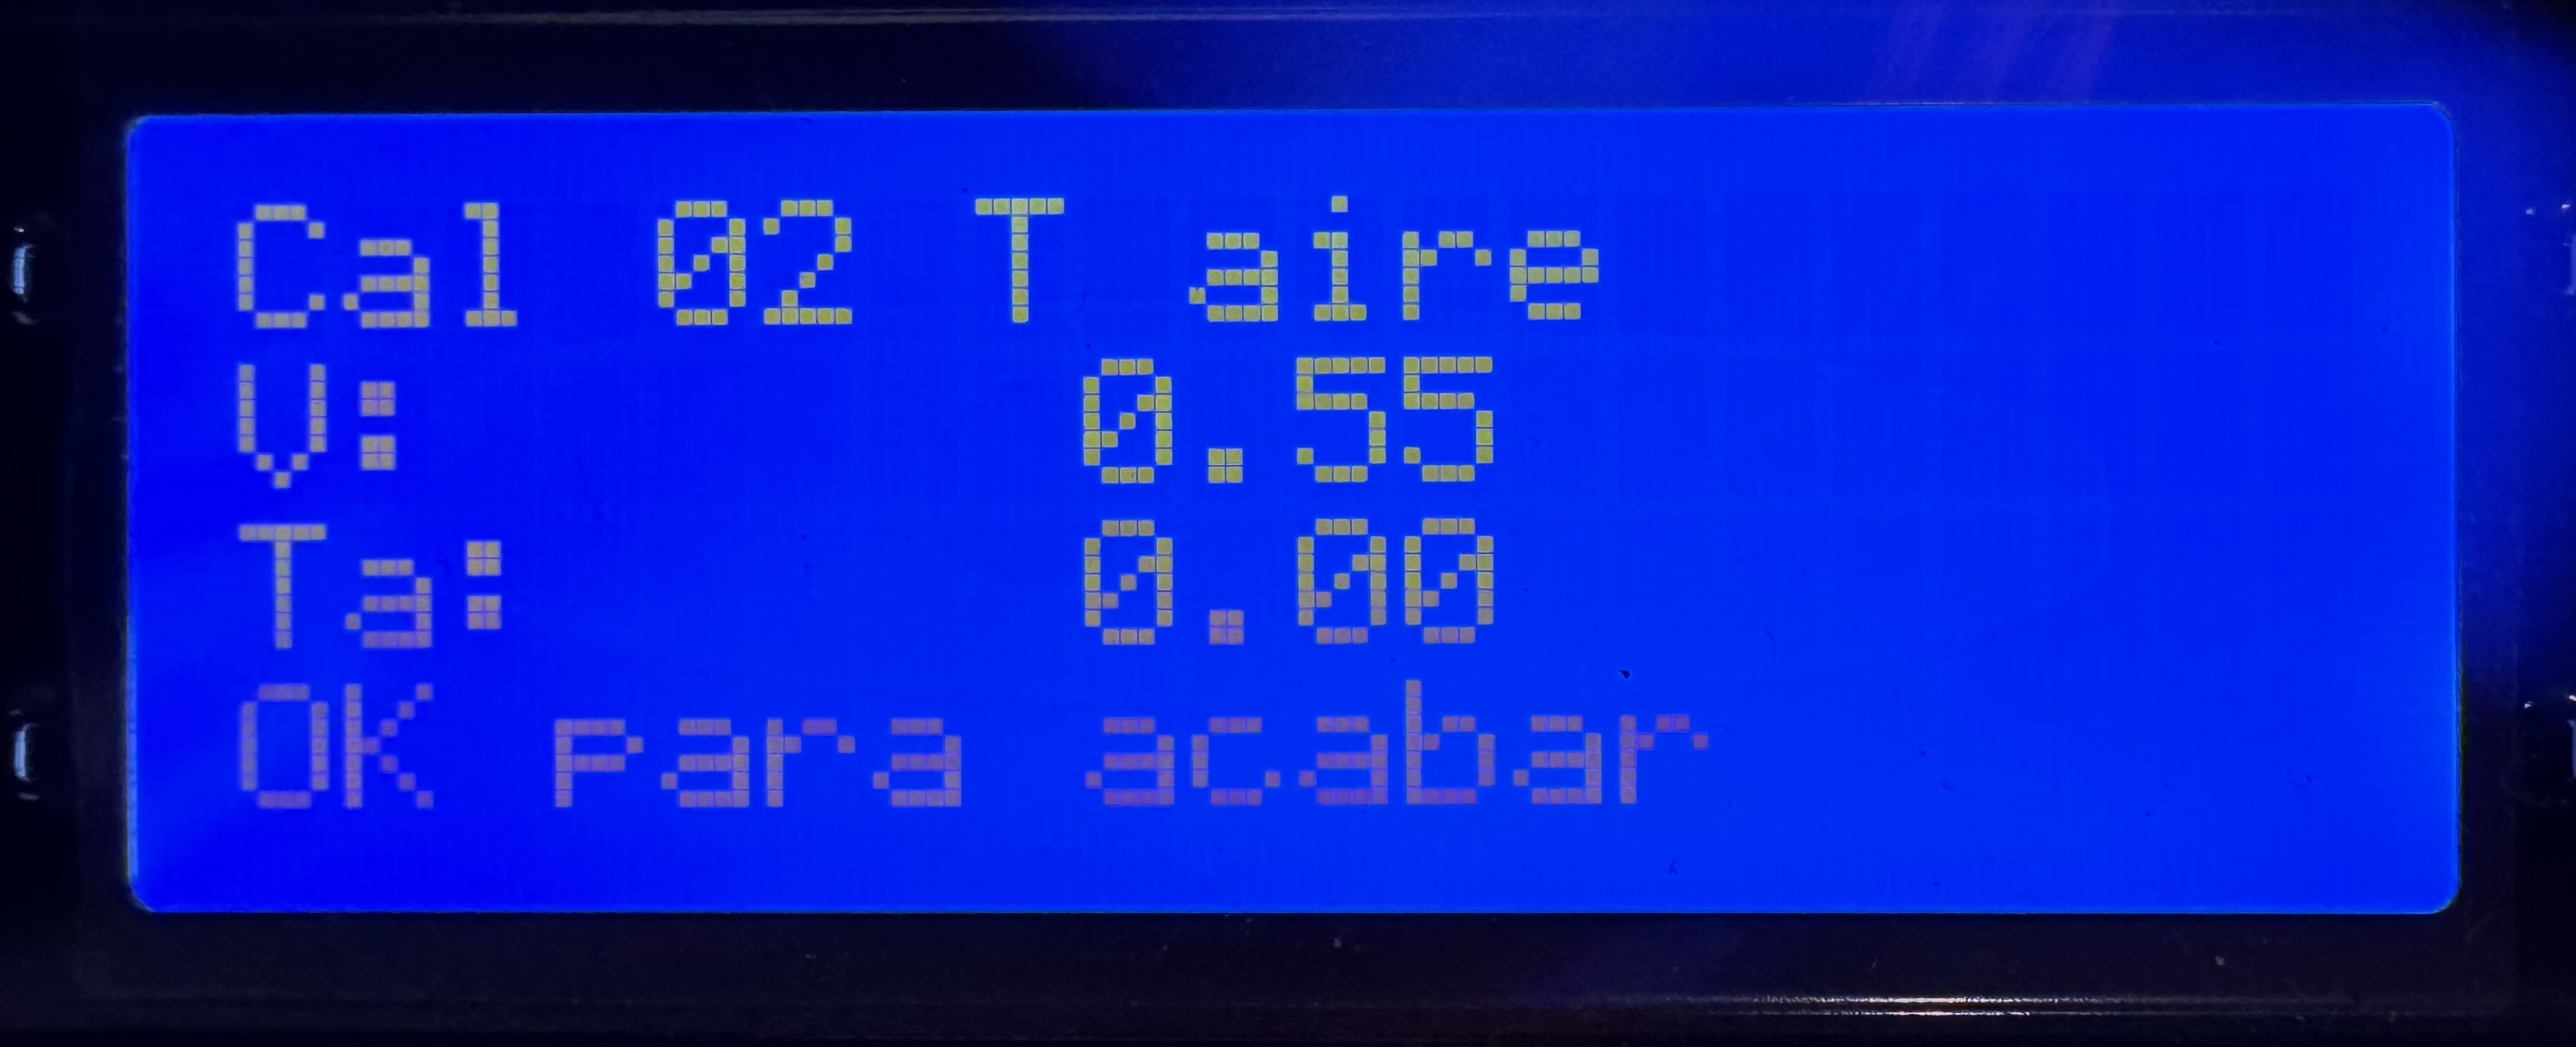
\psfig{file=Figuras/O2aire.jpeg,width=8cm,angle=0}} 
\caption{$1^{er}$ procedimiento para la calibración del sensor de concentración de $O_2$}\label{patalla:O2aire} 
\end{figure}

\begin{itemize}
\item Línea 1: \textbf{Cal 02 T aire}.
\item Línea 2: \textbf{V:} es la tensión que está leyendo el sensor.
\item Línea 3: \textbf{Ta:} El valor de la temperatura del aire proporcionado por el sensor DTH22 conectado el puerto DTH22A. 
\item Línea 4: \textbf{OK para acabar}. Una vez que este todo pulsamos OK para acabar.
\end{itemize}

\item Moja la probeta en agua pura y agítala para que elimine el exceso de agua. Expón la probeta al aire y mantenla en una suave corriente de aire durante un minuto, no uses un ventilador. Cuando el voltaje sea estable pulsa OK. Este procedimiento busca el punto de saturación de oxigeno del agua a una determinada temperatura.

En el archivo \emph{config.txt} se actualizaran los valores \emph{CAL1\_V} y \emph{CAL1\_T}\footnote{Verá que en \emph{config.txt} existen también \emph{CAL2\_V} y \emph{CAL2\_T} para ver al influencia de la temperatura. Pero para ello habría que tener aire a dos temperaturas distintas o agua saturada de O2 a dos temperaturas distintas. Este es el tercer procedimiento que se abandonó por la complejidad del mismo.}.
\end{enumerate}

\subsection{Procedimiento 2. Usando temperatura del agua}
Este es el procedimiento más complicado y el que peores resultados nos ha dado.
\begin{enumerate}
\item Una vez estamos en la pantalla principal pulsamos el botón MODE 4 veces\footnote{Si se pasa la pantalla, siga pulsando hasta que vuelva la pantalla principal} hasta que sale la pantalla (figura \ref{patalla:O2agua}). Fíjese que es la parte superior aparece la frase: \textbf{Cal 02 T agua}.

\begin{figure}[htbp!] 
\centering{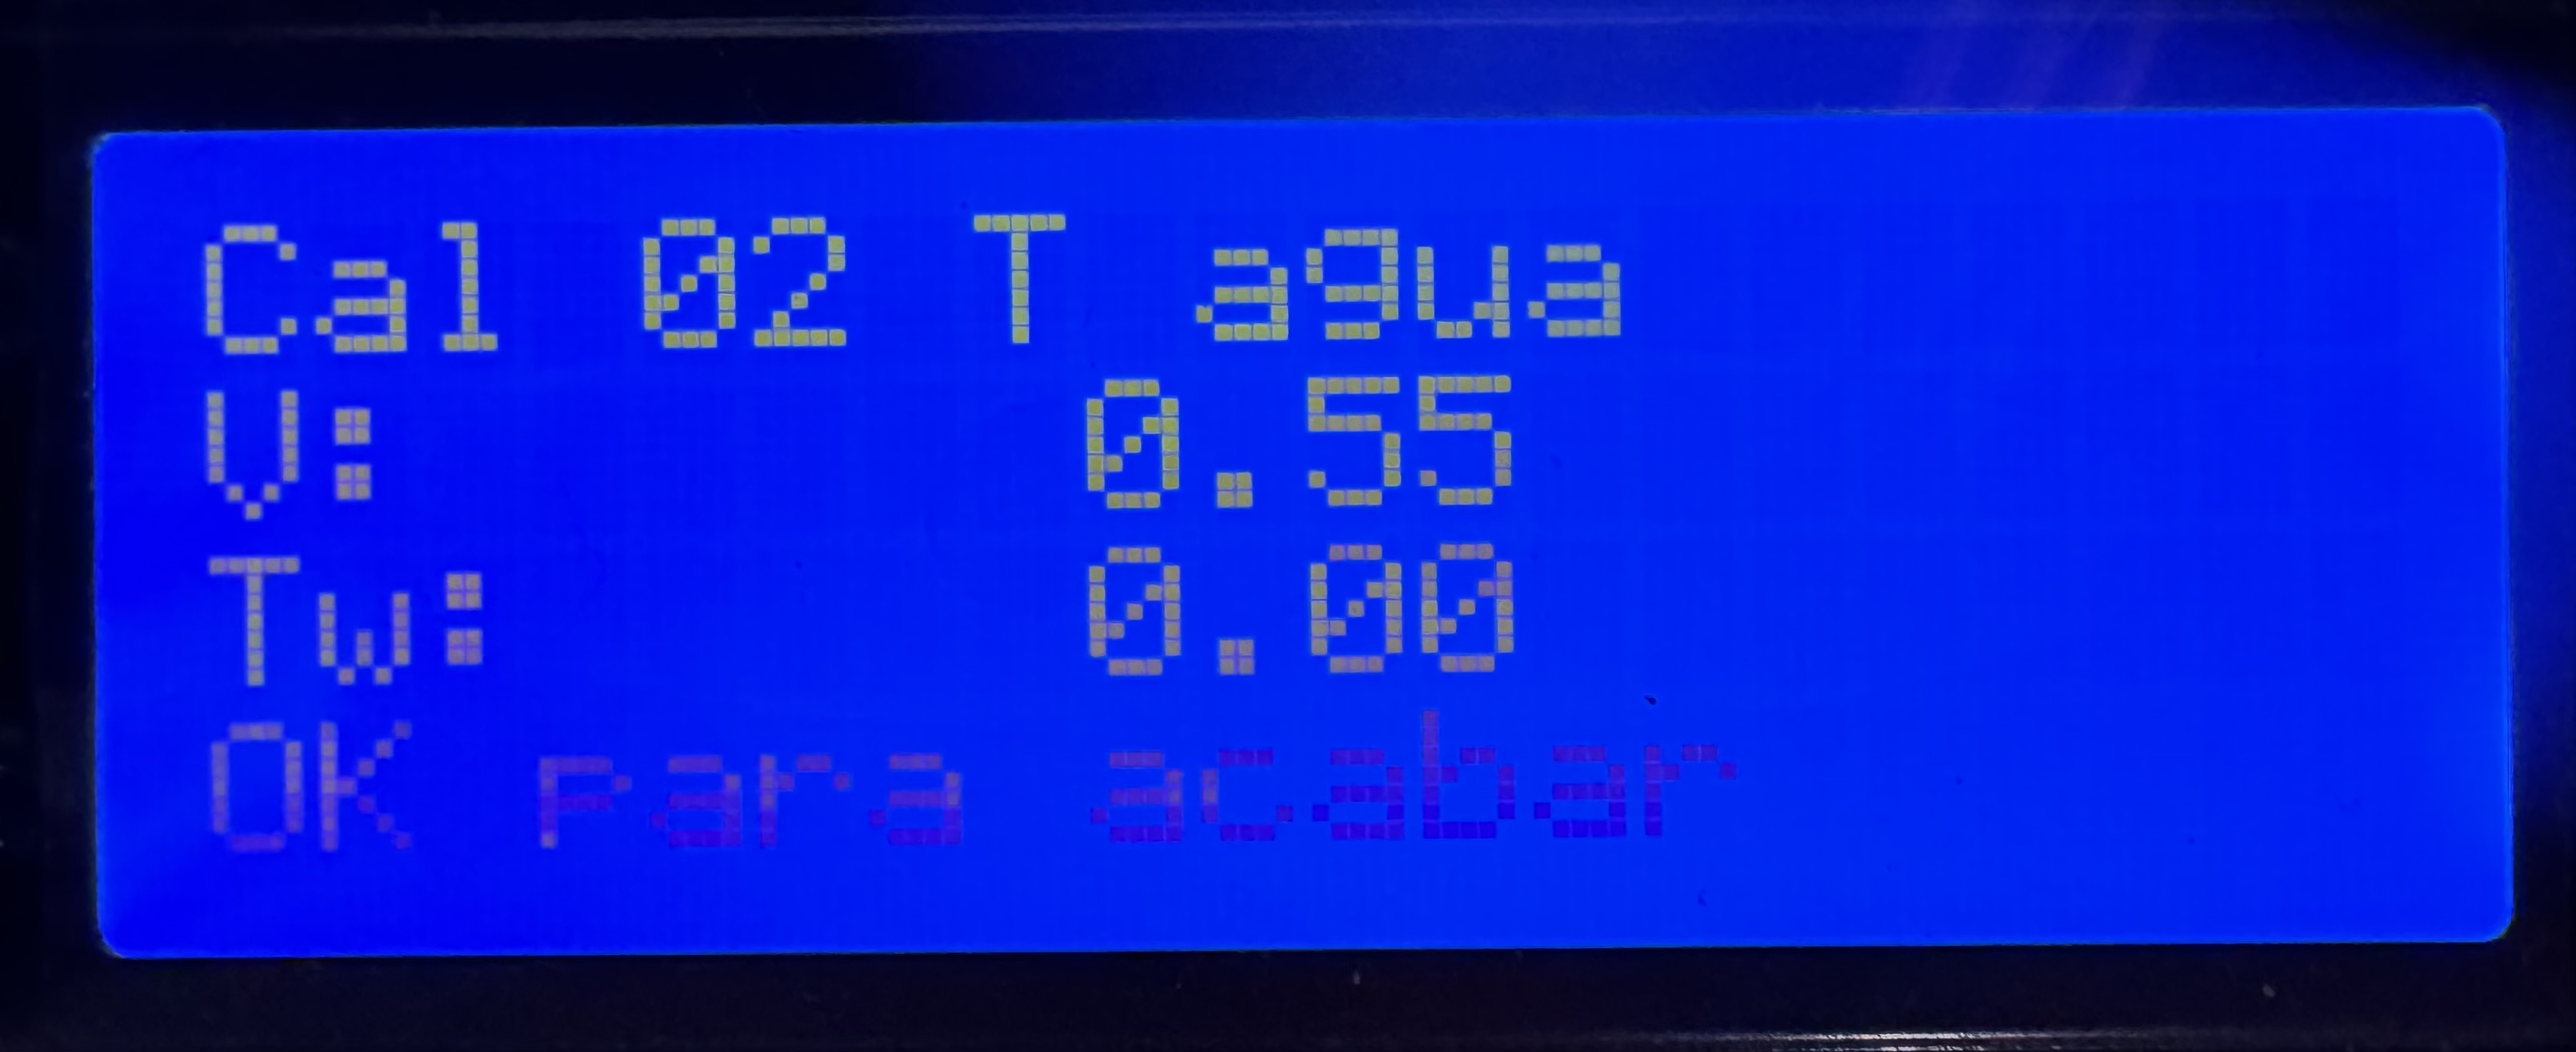
\psfig{file=Figuras/O2agua.jpeg,width=8cm,angle=0}} 
\caption{$2^{\circ}$ procedimiento para la calibración del sensor de concentración de $O_2$}\label{patalla:O2agua} 
\end{figure}

\begin{itemize}
\item Línea 1: \textbf{Cal 02 T aire}.
\item Línea 2: \textbf{V:} es la tensión que está leyendo el sensor.
\item Línea 3: \textbf{Ta:} El valor de la temperatura del agua proporcionado por el sensor DS18B20 (no es el sensor de conductividad).
\item Línea 4: \textbf{OK para acabar}. Una vez que este todo pulsamos OK para acabar.
\end{itemize}

\item Para este procedimiento necesitamos un un baso de agua en el que introducimos una bomba de oxigeno de un acuario. Tenemos que dejar la bomba encendida durante 10 min con objeto de saturar el agua de $O_2$. Una vez hecho esto introducimos la sonda de concentración de $O_2$ y el sensor DS18B20 y esperamos 1 minuto a que al tensión se estabilice. Una vez hecho esto pulsamos OK.

En el archivo \emph{config.txt} se actualizaran los valores \emph{CAL1\_V} y \emph{CAL1\_T}.
\end{enumerate}


\begin{tcolorbox}
[colback=red!5!white,colframe=red!75!black,fonttitle=\bfseries,title=VIDA DEL SENSOR $O_2$]

Según el fabricante la cabeza de la probeta hay que cambiarla cada 4 o 5 meses en caso de agua limpia. La vida de la probeta es de 1 año.

Para ver el procedimiento para cambiar la cabeza de la probeta se puede ver en los link provistos al comienzo de esta sección

\end{tcolorbox}

%%%%%%%%%%%%%%%%%%%%%%%%%%%%%%%%%%%%%%%%%%%%%%%%%%%%%%%%%%%%%%%%%%%%%%%%%%%%%%%%%%%%%%%%%%%%%%%%%%%%%%
\newpage

\section{Sensor de conductividad y calibración}

La conductividad es el recíproco de la resistividad de un objeto. Representa la capacidad de un material para conducir una corriente. En un líquido, la conductividad es una medida de la capacidad de una solución para conducir electricidad y puede reflejar la cantidad de sustancias disueltas o la salinidad de una fuente de agua, por lo que es un parámetro importante en la monitorización de la calidad del agua.

El sensor de conductividad eléctrica analógico Gravity PRO de DFRobot (K=1) SEN0451 está especialmente diseñado para medir la conductividad en soluciones acuosas y así evaluar la calidad del agua. Estos sensores de conductividad se utilizan a menudo en hidroponía, acuicultura, detección ambiental del agua y otros campos.

Como versión mejorada del medidor de conductividad eléctrica analógico, esta versión pro ha mejorado considerablemente la durabilidad de la sonda, lo que permite su uso en la monitorización de la conductividad las 24 horas del día, los 7 días de la semana. Además, el termómetro de resistencia de platino integrado PT1000 facilita la medición de datos de temperatura compensada.

\begin{verbatim}
https://www.dfrobot.com/product-2565.html
https://wiki.dfrobot.com/SKU_SEN0451_Gravity_Analog_Electrical_Conductivity_Sensor_PRO_K_1
\end{verbatim}

La medida de la conductividad es fuertemente dependiente de la temperatura es por eso que la sonda de conductividad viene con una sonda de temperatura incorporada. La sonda de conductividad viene caracterizada por un único parámetro K (ganancia) cuyo valor inicial viene medido de fábrica y que se puede encontrar en el cable de la sonda.

En caso que necesite recalibrar la sonda el procedimiento es sencillo:

Una vez estamos en la pantalla principal pulsamos el botón MODE 5 veces\footnote{Si se pasa la pantalla, siga pulsando hasta que vuelva la pantalla principal} hasta que sale la pantalla (figura \ref{patalla:EC}). Fíjese que es la parte superior aparece la frase: \textbf{Calc EC}.

\begin{figure}[htbp!] 
\centering{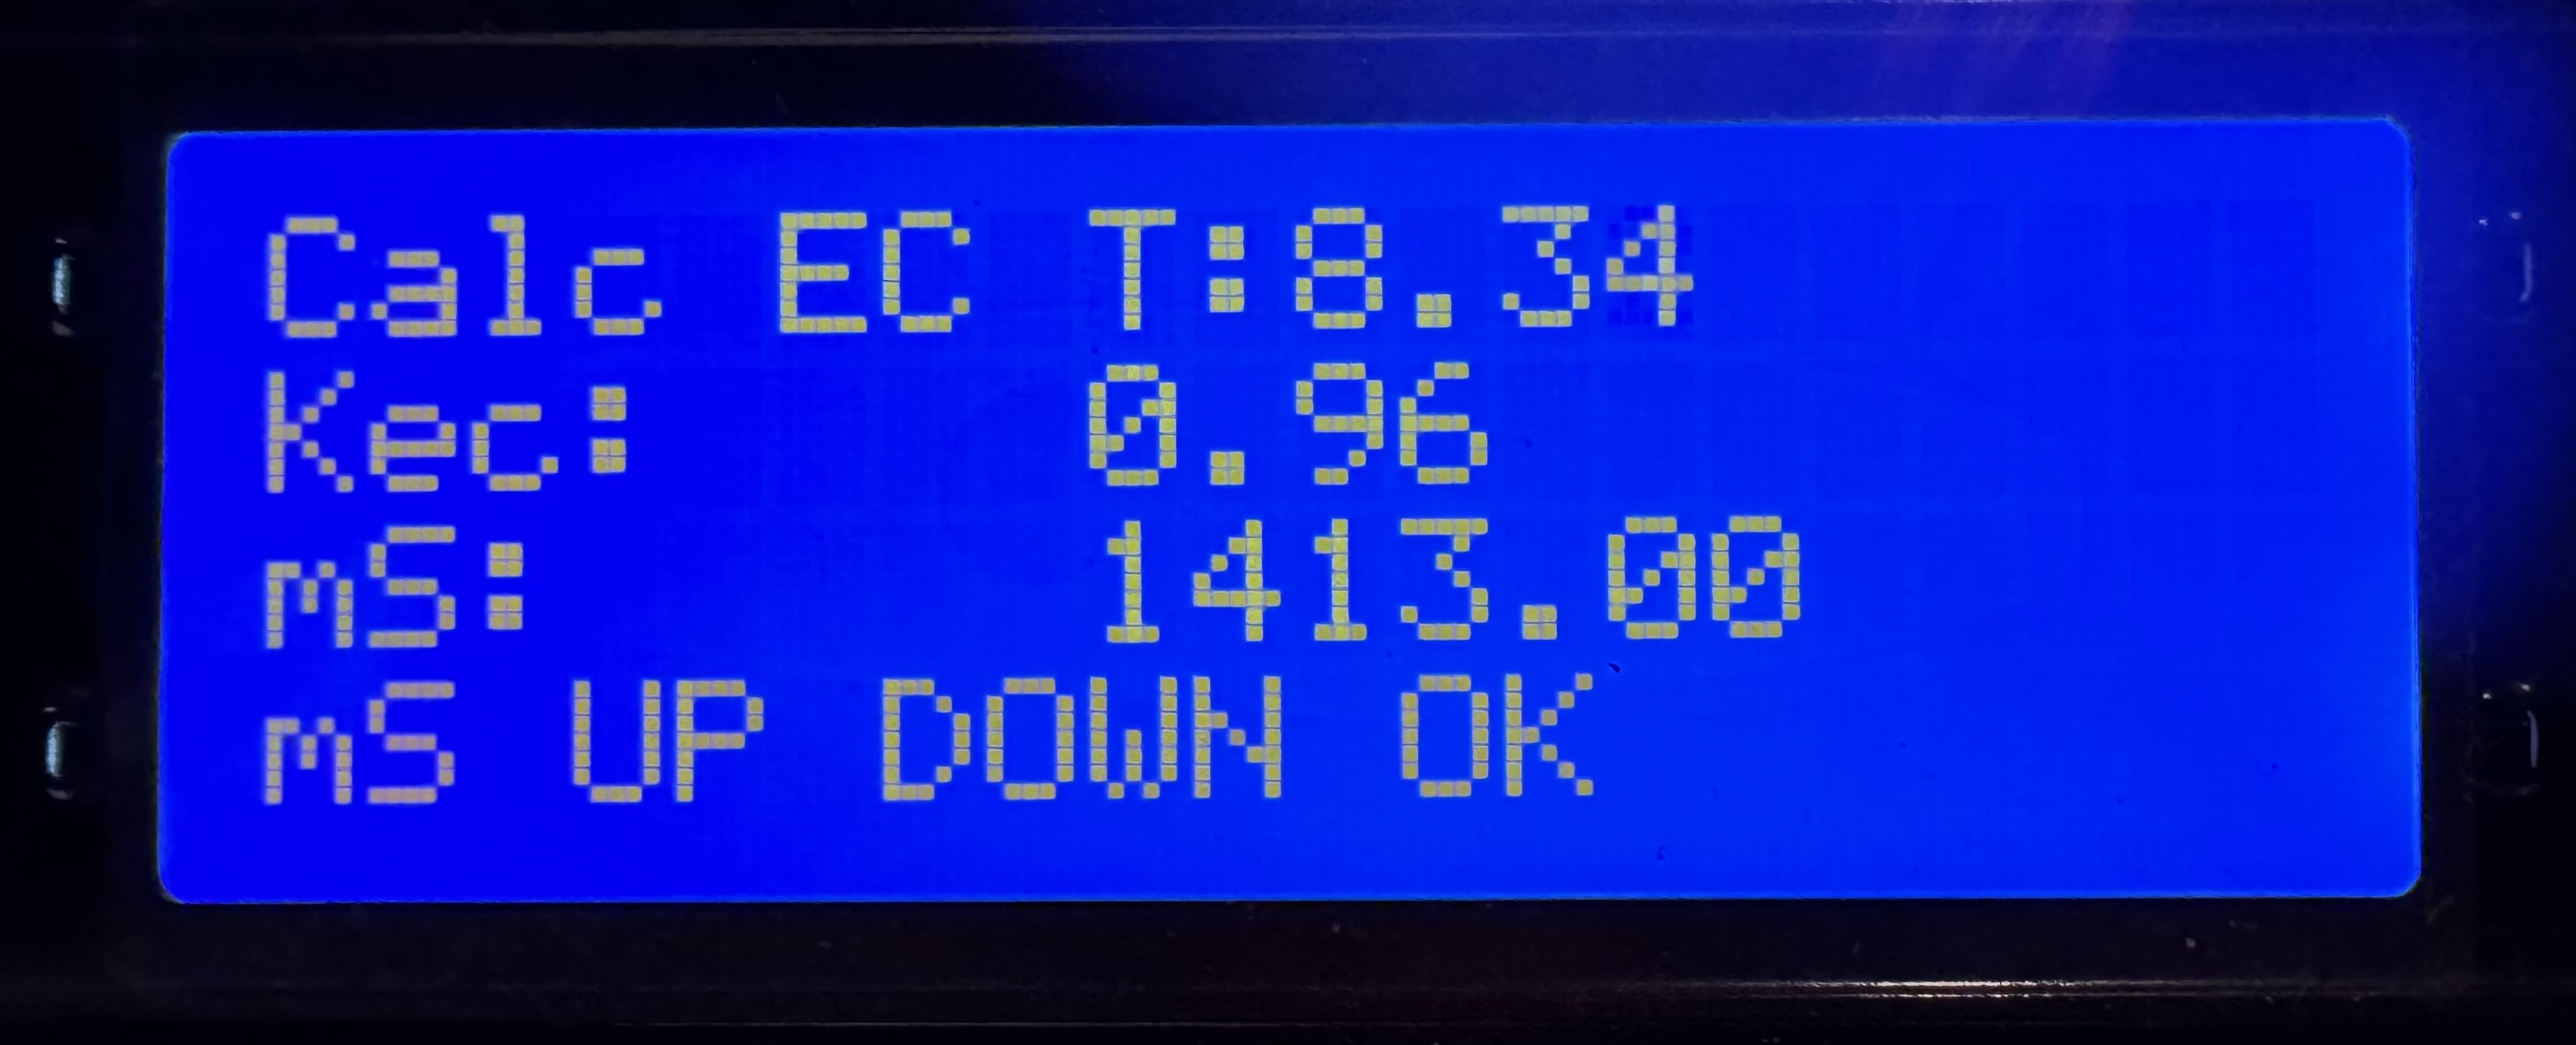
\psfig{file=Figuras/ECcal.jpeg,width=8cm,angle=0}} 
\caption{Procedimiento para la calibración del sensor de conductividad}\label{patalla:EC} 
\end{figure}

\begin{itemize}
\item Línea 1: \textbf{Calc EC} y la temperatura que está leyendo la sonda en ese instante.
\item Línea 2: \textbf{Kec:} es el valor actual de ganancia de la sonda de conductividad.
\item Línea 3: \textbf{mS:} Es el valor de la conductividad de la solución que se usa para calibrar.
\item Línea 4: \textbf{mS UP DOWN OK}. Podemos variar el valor de conductividad de la solución de calibración con UP o DOWN y una vez que este todo pulsamos OK para acabar.
\end{itemize}

El procedimiento es el siguiente: Metemos la probeta del conductividad, previa limpieza, en un líquido de conductividad conocida y \underline{esperamos un minuto} a que se estabilice la tensión. Mientras vamos ajustando el campo mS con UP y DOWN y pulsamos OK.

En el archivo \emph{config.txt} se actualizaran los valores \emph{Kec}, \emph{mS} y \emph{Tec}.

\begin{tcolorbox}
[colback=red!5!white,colframe=red!75!black,fonttitle=\bfseries,title=VIDA DEL SENSOR DE CONDUCTIVIDAD]

El fabricante no da ningún dato ni de cuanto tiempo tiene que pasar entre recalibraciones ni de cuanto es la vida de la probeta por lo que hay que ir haciendo medidas periódicas con otra sonda y comparar.

La probeta que tenemos en el equipo de prueba lleva instalada 3-4 meses y sigue funcionando bien.

\end{tcolorbox}